% Options for packages loaded elsewhere
\PassOptionsToPackage{unicode}{hyperref}
\PassOptionsToPackage{hyphens}{url}
%
\documentclass[
  openany]{book}
\usepackage{amsmath,amssymb}
\usepackage{lmodern}
\usepackage{iftex}
\ifPDFTeX
  \usepackage[T1]{fontenc}
  \usepackage[utf8]{inputenc}
  \usepackage{textcomp} % provide euro and other symbols
\else % if luatex or xetex
  \usepackage{unicode-math}
  \defaultfontfeatures{Scale=MatchLowercase}
  \defaultfontfeatures[\rmfamily]{Ligatures=TeX,Scale=1}
\fi
% Use upquote if available, for straight quotes in verbatim environments
\IfFileExists{upquote.sty}{\usepackage{upquote}}{}
\IfFileExists{microtype.sty}{% use microtype if available
  \usepackage[]{microtype}
  \UseMicrotypeSet[protrusion]{basicmath} % disable protrusion for tt fonts
}{}
\makeatletter
\@ifundefined{KOMAClassName}{% if non-KOMA class
  \IfFileExists{parskip.sty}{%
    \usepackage{parskip}
  }{% else
    \setlength{\parindent}{0pt}
    \setlength{\parskip}{6pt plus 2pt minus 1pt}}
}{% if KOMA class
  \KOMAoptions{parskip=half}}
\makeatother
\usepackage{xcolor}
\IfFileExists{xurl.sty}{\usepackage{xurl}}{} % add URL line breaks if available
\IfFileExists{bookmark.sty}{\usepackage{bookmark}}{\usepackage{hyperref}}
\hypersetup{
  pdftitle={scRNA-seq data analysis},
  pdfauthor={David Chisanga and Wei Shi},
  hidelinks,
  pdfcreator={LaTeX via pandoc}}
\urlstyle{same} % disable monospaced font for URLs
\usepackage{color}
\usepackage{fancyvrb}
\newcommand{\VerbBar}{|}
\newcommand{\VERB}{\Verb[commandchars=\\\{\}]}
\DefineVerbatimEnvironment{Highlighting}{Verbatim}{commandchars=\\\{\}}
% Add ',fontsize=\small' for more characters per line
\usepackage{framed}
\definecolor{shadecolor}{RGB}{248,248,248}
\newenvironment{Shaded}{\begin{snugshade}}{\end{snugshade}}
\newcommand{\AlertTok}[1]{\textcolor[rgb]{0.94,0.16,0.16}{#1}}
\newcommand{\AnnotationTok}[1]{\textcolor[rgb]{0.56,0.35,0.01}{\textbf{\textit{#1}}}}
\newcommand{\AttributeTok}[1]{\textcolor[rgb]{0.77,0.63,0.00}{#1}}
\newcommand{\BaseNTok}[1]{\textcolor[rgb]{0.00,0.00,0.81}{#1}}
\newcommand{\BuiltInTok}[1]{#1}
\newcommand{\CharTok}[1]{\textcolor[rgb]{0.31,0.60,0.02}{#1}}
\newcommand{\CommentTok}[1]{\textcolor[rgb]{0.56,0.35,0.01}{\textit{#1}}}
\newcommand{\CommentVarTok}[1]{\textcolor[rgb]{0.56,0.35,0.01}{\textbf{\textit{#1}}}}
\newcommand{\ConstantTok}[1]{\textcolor[rgb]{0.00,0.00,0.00}{#1}}
\newcommand{\ControlFlowTok}[1]{\textcolor[rgb]{0.13,0.29,0.53}{\textbf{#1}}}
\newcommand{\DataTypeTok}[1]{\textcolor[rgb]{0.13,0.29,0.53}{#1}}
\newcommand{\DecValTok}[1]{\textcolor[rgb]{0.00,0.00,0.81}{#1}}
\newcommand{\DocumentationTok}[1]{\textcolor[rgb]{0.56,0.35,0.01}{\textbf{\textit{#1}}}}
\newcommand{\ErrorTok}[1]{\textcolor[rgb]{0.64,0.00,0.00}{\textbf{#1}}}
\newcommand{\ExtensionTok}[1]{#1}
\newcommand{\FloatTok}[1]{\textcolor[rgb]{0.00,0.00,0.81}{#1}}
\newcommand{\FunctionTok}[1]{\textcolor[rgb]{0.00,0.00,0.00}{#1}}
\newcommand{\ImportTok}[1]{#1}
\newcommand{\InformationTok}[1]{\textcolor[rgb]{0.56,0.35,0.01}{\textbf{\textit{#1}}}}
\newcommand{\KeywordTok}[1]{\textcolor[rgb]{0.13,0.29,0.53}{\textbf{#1}}}
\newcommand{\NormalTok}[1]{#1}
\newcommand{\OperatorTok}[1]{\textcolor[rgb]{0.81,0.36,0.00}{\textbf{#1}}}
\newcommand{\OtherTok}[1]{\textcolor[rgb]{0.56,0.35,0.01}{#1}}
\newcommand{\PreprocessorTok}[1]{\textcolor[rgb]{0.56,0.35,0.01}{\textit{#1}}}
\newcommand{\RegionMarkerTok}[1]{#1}
\newcommand{\SpecialCharTok}[1]{\textcolor[rgb]{0.00,0.00,0.00}{#1}}
\newcommand{\SpecialStringTok}[1]{\textcolor[rgb]{0.31,0.60,0.02}{#1}}
\newcommand{\StringTok}[1]{\textcolor[rgb]{0.31,0.60,0.02}{#1}}
\newcommand{\VariableTok}[1]{\textcolor[rgb]{0.00,0.00,0.00}{#1}}
\newcommand{\VerbatimStringTok}[1]{\textcolor[rgb]{0.31,0.60,0.02}{#1}}
\newcommand{\WarningTok}[1]{\textcolor[rgb]{0.56,0.35,0.01}{\textbf{\textit{#1}}}}
\usepackage{longtable,booktabs,array}
\usepackage{calc} % for calculating minipage widths
% Correct order of tables after \paragraph or \subparagraph
\usepackage{etoolbox}
\makeatletter
\patchcmd\longtable{\par}{\if@noskipsec\mbox{}\fi\par}{}{}
\makeatother
% Allow footnotes in longtable head/foot
\IfFileExists{footnotehyper.sty}{\usepackage{footnotehyper}}{\usepackage{footnote}}
\makesavenoteenv{longtable}
\usepackage{graphicx}
\makeatletter
\def\maxwidth{\ifdim\Gin@nat@width>\linewidth\linewidth\else\Gin@nat@width\fi}
\def\maxheight{\ifdim\Gin@nat@height>\textheight\textheight\else\Gin@nat@height\fi}
\makeatother
% Scale images if necessary, so that they will not overflow the page
% margins by default, and it is still possible to overwrite the defaults
% using explicit options in \includegraphics[width, height, ...]{}
\setkeys{Gin}{width=\maxwidth,height=\maxheight,keepaspectratio}
% Set default figure placement to htbp
\makeatletter
\def\fps@figure{htbp}
\makeatother
\setlength{\emergencystretch}{3em} % prevent overfull lines
\providecommand{\tightlist}{%
  \setlength{\itemsep}{0pt}\setlength{\parskip}{0pt}}
\setcounter{secnumdepth}{5}
\usepackage{booktabs}
\usepackage{amsthm}
\makeatletter
\def\thm@space@setup{%
  \thm@preskip=4pt plus 2pt minus 4pt
  \thm@postskip=\thm@preskip
}
\makeatother
\usepackage{pdflscape}
\newcommand{\blandscape}{\begin{landscape}}
\newcommand{\elandscape}{\end{landscape}}
\ifLuaTeX
  \usepackage{selnolig}  % disable illegal ligatures
\fi
\usepackage[]{natbib}
\bibliographystyle{apalike}

\title{scRNA-seq data analysis}
\author{David Chisanga and Wei Shi}
\date{24 June, 2022}

\begin{document}
\maketitle

{
\setcounter{tocdepth}{1}
\tableofcontents
}
\hypertarget{preface}{%
\chapter{Preface}\label{preface}}

This tutorial describes the Bioinformatics protocol for analyzing single-cell RNA-seq (scRNA-seq) data using \href{https://rdrr.io/bioc/Rsubread/man/cellCounts.html}{\emph{cellCounts}} function in (\textbf{Rsubread}) and \textbf{Seurat} pipeline. This guide provides a brief discussion and examples of the steps involved in the analysis of scRNA-seq data. These include;

\begin{itemize}
\tightlist
\item
  processing raw data,
\item
  quality control,
\item
  normalization,
\item
  data correction,
\item
  dimension reduction,
\item
  cluster analysis,
\item
  cell type annotation,
\item
  trajectory analysis
\item
  and other downstream analyses.
\end{itemize}

\vspace{-100pt}

\vspace{-100pt}

\hypertarget{intro}{%
\chapter{Introduction}\label{intro}}

Single-cell RNA-seq (scRNA-seq) first published by \citep{tang2009mrna} measures the distribution of expression levels in individual cells. This allows for the study of transcriptome changes at the cellular level to provide unprecedented resolution of gene expression changes in complex cellular systems. As in bulk RNA-seq, scRNA-seq involves a range of analyses including quantification, dimension reduction, cell clustering, cell type identification, inference of gene-regulatory networks, differential expression and cell hierarchy reconstruction. This scRNA-seq protocol provides a step-by-step overview of a standard scRNA-seq analysis. The steps can be categorized into 3 groups; quantification, quality control and downstream analysis

\begin{landscape}
\begin{figure}

{\centering 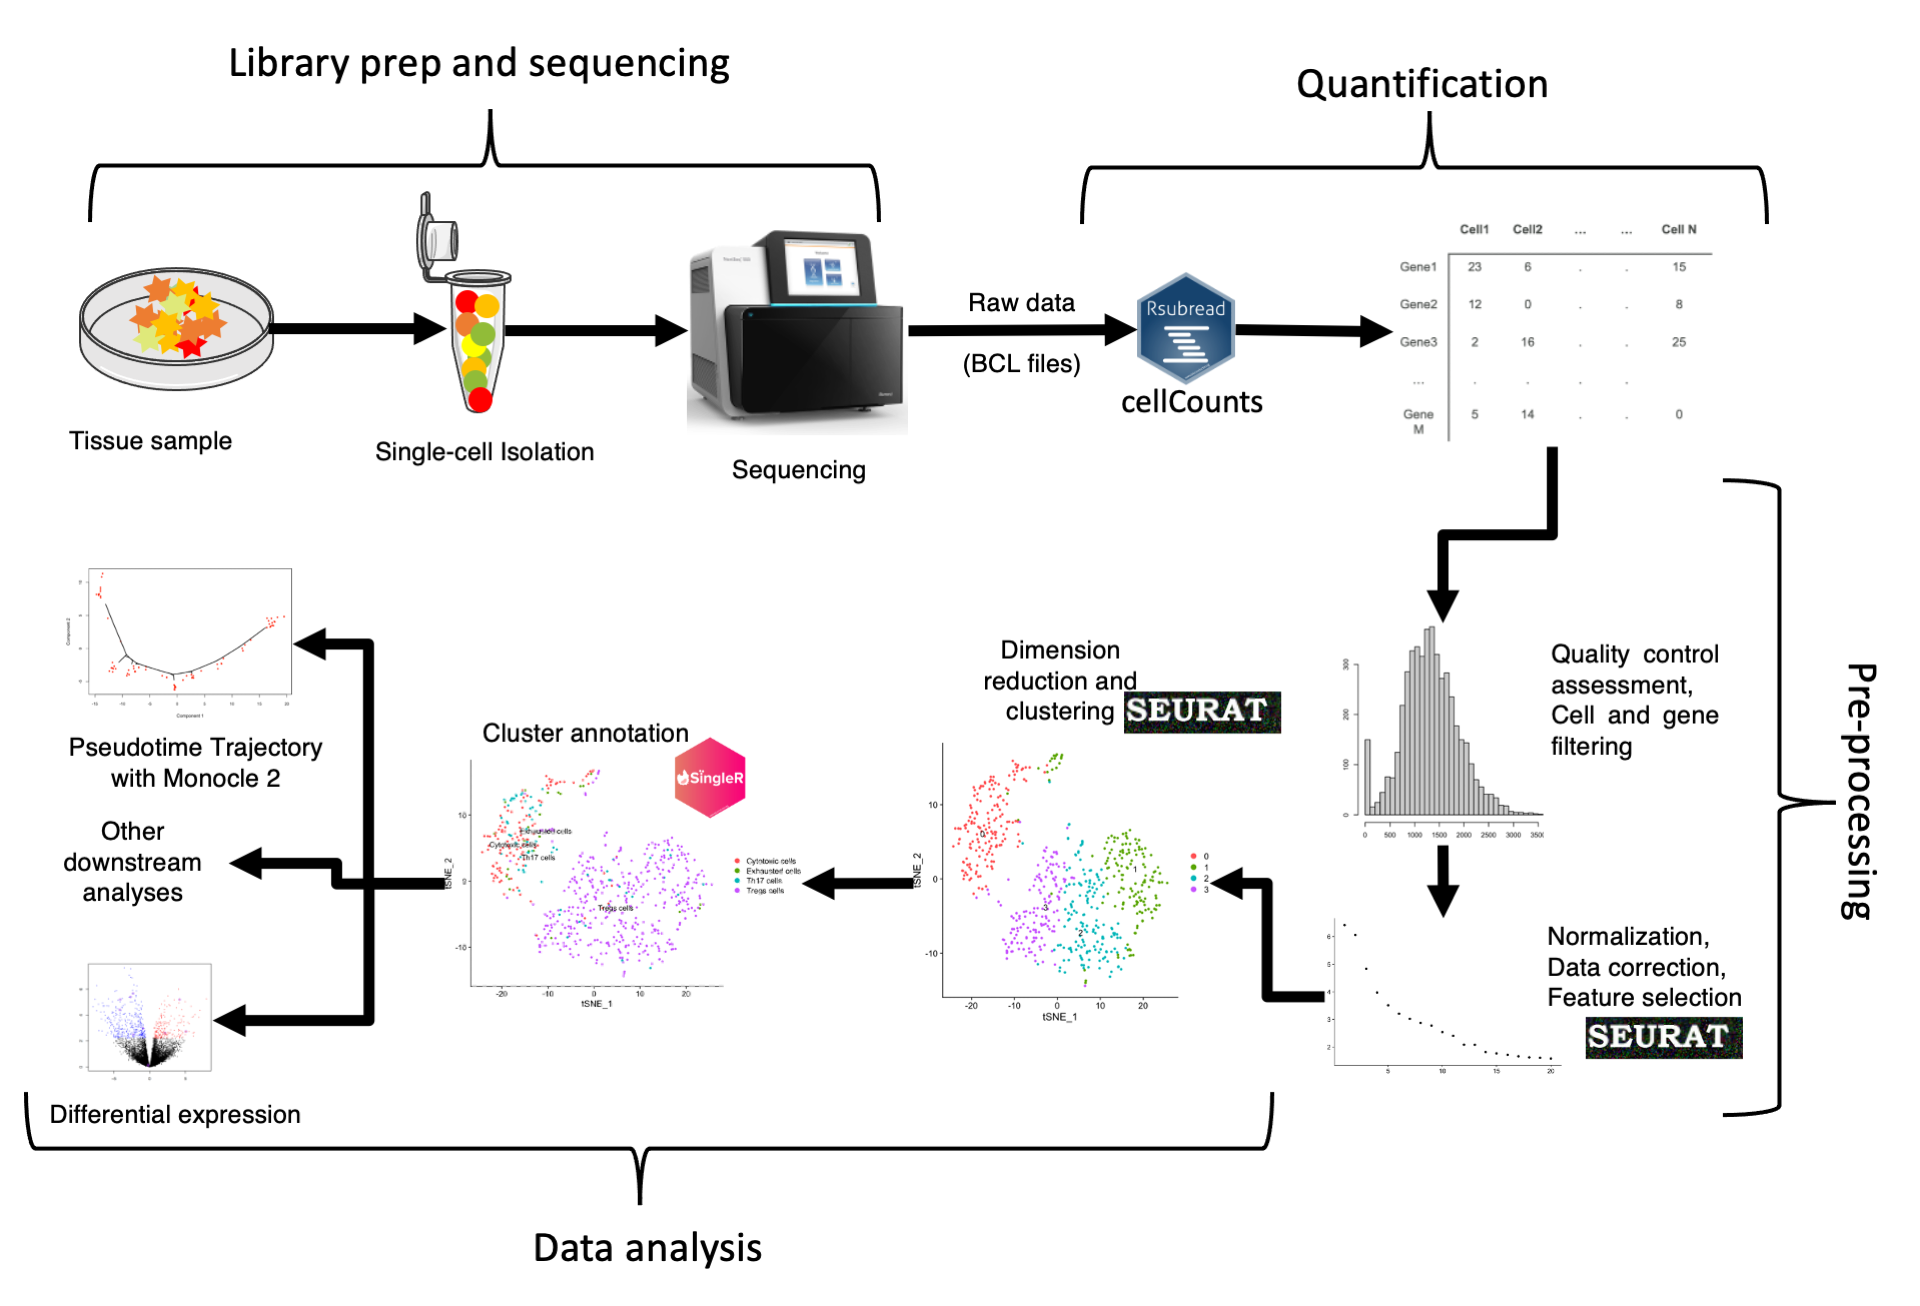
\includegraphics[width=26.67in]{Fig1} 

}

\caption{Overview of the scRNA-seq analysis protocol}\label{fig:fig1}
\end{figure}
\end{landscape}

\hypertarget{quantification}{%
\section{Quantification}\label{quantification}}

Converting the raw data into a matrix of counts is the first step in a scRNA-seq analysis. \emph{cellCounts} a scRNA-seq quantification program within \textbf{Rsubread} is used in the quantification step. \href{https://rdrr.io/bioc/Rsubread/man/cellCounts.html}{\textbf{cellCounts}} is a program developed for quantifying single-cell RNA-seq (scRNA-seq) data generated from the \href{https://www.10xgenomics.com/products/single-cell-gene-expression}{10X platform}. cellCounts takes as input scRNA-seq reads, maps them to the reference genome and then produces UMI (Unique Molecular Identifier) counts for each gene in each cell. Its read mapping is based on the \textbf{align} program \citep{Rsubread2019, liao2013subread} and its UMI counting is based on the \emph{featureCounts} program \citep{liao2013featurecounts}. Sample demultiplexing, cell barcode demultiplexing and read deduplication are carried out before generating the UMI counts.

The \emph{cellCounts} function returns a R list object which contains the following components:

\textbf{counts}\\
A List object including UMI counts for each sample. Each component in this object is a matrix that contains UMI counts for a sample. Rows in the matrix are genes and columns are cells.

\textbf{annotation}\\
A data.frame object containing a gene annotation. This is the annotation that was used for the assignment of UMIs to genes during quantification. Rows in the annotation are genes. Columns of the annotation include GeneID, Chr, Start, End and Length.

\textbf{sample.info}\\
A data.frame object containing sample information and quantification statistics. It includes the following columns: SampleName, InputDirectory (if the input format is BCL), TotalCells,HighConfidenceCells (if umi.cutoff is NULL), RescuedCells (if umi.cutoff is NULL), TotalUMI, MinUMI, MedianUMI, MaxUMI, MeanUMI, TotalReads, MappedReads and AssignedReads. Each row in the data frame is a sample.

\textbf{cell.confidence}\\
A List object indicating if a cell is a high-confidence cell or a rescued cell (low confidence). Each component in the object is a logical vector indicating which cells in a sample are high-confidence cells. cell confidence is included in the output only if umi cutoff is NULL.

\hypertarget{quality-control-and-normalization}{%
\section{Quality control and Normalization}\label{quality-control-and-normalization}}

This step largely consists of quality control, normalization, data correction and dimension reduction. For this step, we will use visualization plots and utilize a number of functions within the \textbf{Seurat} \citep{hao2021} pipeline for scRNA-seq analysis.

\hypertarget{quality-control}{%
\subsection{Quality control}\label{quality-control}}

\textbf{Cell filtering}\\

Quality control is performed in several ways to remove;

\begin{itemize}
\tightlist
\item
  low quality cells
\item
  contaminants
\end{itemize}

A number of metrics are used to assess the quality of the scRNA-seq data including the proportion of detected genes in each cell, and fraction of UMI accounts associated with Mitochondrial/Ribosomal genes.

Cells with a low or high number of detected genes are indicative of

\begin{itemize}
\tightlist
\item
  quiescent/damaged cells or
\item
  doublets/multiplets \citep{nayak2021hitchhiker}
\end{itemize}

A high fraction of mitochondrial genes in a cell is associated with \href{https://kb.10xgenomics.com/hc/en-us/articles/360001086611-Why-do-I-see-a-high-level-of-mitochondrial-gene-expression-}{(See 10X website)}

\begin{itemize}
\tightlist
\item
  poor sample quality which leads to a high fraction of apoptotic or lysing cells.
\item
  biology of the particular sample, for example, tumor biopsies, may have increased mitochondrial gene expression due to metabolic activity and/or necrosis.
\end{itemize}

A high fraction of ribosomal genes in each cell is indicative of RNA degradation which leads to more templating of rRNA-fragments \href{https://kb.10xgenomics.com/hc/en-us/articles/218169723-What-fraction-of-reads-map-to-ribosomal-proteins-}{(See 10X website)}

To decide what cut-offs to use, we will visualize the distributions of each metric using plots such as histograms and box plots.

\textbf{Gene filtering}\\

Genes not meeting the following criteria are also filtered;

\begin{itemize}
\tightlist
\item
  Genes not expressed in at least a given number of cells
\item
  Genes that may have very high expression
\item
  Mitochondrial encoded genes
\item
  Ribosomal encoded genes
\item
  Genes deemed to induce technical bias
\end{itemize}

\hypertarget{normalisation-and-data-correction}{%
\subsection{Normalisation and data correction}\label{normalisation-and-data-correction}}

The filtered count matrix is normalized to account for gene expression variability between cells. There are several normalization methods, a number of which have been derived from Bulk RNA-seq and include;

\begin{itemize}
\tightlist
\item
  CPM (Counts Per Million)
\item
  TPM (Transcripts Per Million)
\item
  FPKM (Fragments Per Kilobase Million)
\item
  TMM (Trimmed Mean of M-values)
\item
  Quantile normalization
\end{itemize}

The sparsity and high heterogeneity in scRNA-seq adds to the complexity of normalizing scRNA-seq data. Here, we will utilize normalization methods included in the \textbf{Seurat} package. We will be using a global-scaling normalization method ``LogNormalize'' in \textbf{Seurat}, this method normalizes the feature expression measurements for each cell by the total expression, multiplies this by a scale factor (10,000 by default), and log-transforms the result. In addition, for Differential Expression analysis, we utilize the the limma-voom pipeline \citep[law2014voom]{ritchie2015limma} and here, we will be using the CPM normalization method.

\hypertarget{dimension-reduction}{%
\subsection{Dimension reduction}\label{dimension-reduction}}

The resulting count matrix from scRNA-seq is high dimensional in nature. Furthermore, not all the genes included in the matrix are needed for the classification of the cellular expression profiles. As such, it is important that we focus on the Biological signals that are informative. Popular techniques for dimension reduction are;

\begin{itemize}
\tightlist
\item
  PCA (Principal Component Analysis)
\item
  t-distributed Stochastic Neighbor Embedding (t-SNE)
\item
  Uniform Manifold Approximation, and Projection (UMAP)
\item
  Self Organizing Maps (SOM)
\end{itemize}

There are two components involved in dimension reduction;

\begin{itemize}
\tightlist
\item
  Feature selection where a small subset of features is selected
\item
  Feature extraction where higher dimension data is projected to a lower dimension
\end{itemize}

In this workshop, t-SNE and UMAP are used to demonstrate how to group cells into clusters.

\hypertarget{data-analysis}{%
\section{Data analysis}\label{data-analysis}}

After the data has been processed, there are several analyses that can be done depending on the research question. In this tutorial, we will look at the standard analysis in scRNA-seq such as Cluster analysis, cell type annotation, and Trajectory inference/pseudo-temporal ordering. We will also perform gene-level analysis including differential expression analysis, pathway and gene set enrichment analysis, and the generation of Gene Regulatory Networks
\vspace{-100pt}

\vspace{-100pt}

\hypertarget{prerequisites}{%
\chapter{Prerequisites}\label{prerequisites}}

Before you get started with the rest of the analysis, it is important that you have the necessary data and software that will be used in this analysis.

\hypertarget{prereq}{%
\section{Data}\label{prereq}}

\textbf{scRNA-seq data}\\

A subset of the scRNA-seq dataset that was generated in a published study \citep{chen2020multicenter} is used as an example dataset in this protocol. The data consists of two well-characterized cellular reference samples (human breast cancer cell line (HCC1395, sample A) and the matched normal B lymphocyte line (HCC1395BL, sample B)) that were captured using the 10X platform. The data is available in the SRA repository under accession code no. \href{https://www.ncbi.nlm.nih.gov/bioproject/?term=PRJNA504037}{PRJNA504037}. However, for the convenience of this analysis, FASTQ files of the raw scRNA-seq data were also saved in the `Workshop\_scRNAseq' directory on the Z drive.

A text file called ``targets.csv'', which includes relevant sample information can also be found in this directory.

\textbf{Reference genome data}\\

A FASTA-format file including all chromosomal sequences of the GRCh38/hg38 genome was also saved in the `Workshop\_scRNAseq' directory on Z drive.

\hypertarget{software}{%
\section{SOFTWARE}\label{software}}

The following software tools should be installed on the UNIX server and on your laptop:

\begin{itemize}
\tightlist
\item
  \href{https://www.r-project.org}{R}
\item
  \href{http://bioconductor.org/packages/release/bioc/html/Rsubread.html}{Rsubread}
\item
  \href{http://bioconductor.org/packages/release/bioc/html/limma.html}{limma}
\item
  \href{http://bioconductor.org/packages/release/bioc/html/edgeR.html}{edgeR}
\item
  \href{http://bioconductor.org/packages/release/data/annotation/html/org.Hs.eg.db.html}{org.Hs.eg.db}
\item
  \href{https://CRAN.R-project.org/package=statmod}{statmod}
\item
  \href{https://cloud.r-project.org/package=Seurat}{Seurat}
\item
  \href{https://bioconductor.org/packages/release/bioc/html/SingleR.html}{SingleR}
\item
  \href{https://bioconductor.org/packages/release/bioc/html/monocle.html}{monocle}
\end{itemize}

Consult the R Project website for the installation of R (\url{https://www.r-project.org/}) \citep{R-base}. Make sure the latest release version of R is downloaded and installed. After R is installed, launch R and type the following commands to install \emph{Rsubread}, \emph{limma}, \emph{edgeR}, \emph{org.Hs.eg.db}, \emph{statmod}, \emph{Seurat}, \emph{SingleR} and \emph{Monocle}:

\begin{Shaded}
\begin{Highlighting}[]
\ControlFlowTok{if}\NormalTok{ (}\SpecialCharTok{!}\FunctionTok{requireNamespace}\NormalTok{(}\StringTok{"BiocManager"}\NormalTok{, }\AttributeTok{quietly =} \ConstantTok{TRUE}\NormalTok{))}
  \FunctionTok{install.packages}\NormalTok{(}\StringTok{"BiocManager"}\NormalTok{)}
\NormalTok{BiocManager}\SpecialCharTok{::}\FunctionTok{install}\NormalTok{(}
  \FunctionTok{c}\NormalTok{(}
    \StringTok{\textquotesingle{}Rsubread\textquotesingle{}}\NormalTok{,}
    \StringTok{"org.Hs.eg.db"}\NormalTok{,}
    \StringTok{"SingleR"}\NormalTok{,}
    \StringTok{\textquotesingle{}BiocGenerics\textquotesingle{}}\NormalTok{,}
    \StringTok{\textquotesingle{}DelayedArray\textquotesingle{}}\NormalTok{,}
    \StringTok{\textquotesingle{}DelayedMatrixStats\textquotesingle{}}\NormalTok{,}
    \StringTok{\textquotesingle{}S4Vectors\textquotesingle{}}\NormalTok{,}
    \StringTok{\textquotesingle{}SingleCellExperiment\textquotesingle{}}\NormalTok{,}
    \StringTok{\textquotesingle{}limma\textquotesingle{}}\NormalTok{,}
    \StringTok{\textquotesingle{}edgeR\textquotesingle{}}\NormalTok{,}
    \StringTok{\textquotesingle{}SummarizedExperiment\textquotesingle{}}\NormalTok{,}
    \StringTok{\textquotesingle{}batchelor\textquotesingle{}}\NormalTok{,}
    \StringTok{\textquotesingle{}Matrix.utils\textquotesingle{}}\NormalTok{,}
    \StringTok{\textquotesingle{}monocle\textquotesingle{}}\NormalTok{,}
    \StringTok{\textquotesingle{}celldex\textquotesingle{}}
\NormalTok{  ),}
  \AttributeTok{update =}\NormalTok{ T}
\NormalTok{)}

\ControlFlowTok{if}\NormalTok{ (}\SpecialCharTok{!}\FunctionTok{requireNamespace}\NormalTok{(}\StringTok{"statmod"}\NormalTok{, }\AttributeTok{quietly =} \ConstantTok{TRUE}\NormalTok{))}
  \FunctionTok{install.packages}\NormalTok{(}\StringTok{"statmod"}\NormalTok{)}
\ControlFlowTok{if}\NormalTok{ (}\SpecialCharTok{!}\FunctionTok{requireNamespace}\NormalTok{(}\StringTok{"Seurat"}\NormalTok{, }\AttributeTok{quietly =} \ConstantTok{TRUE}\NormalTok{))}
  \FunctionTok{install.packages}\NormalTok{(}\StringTok{"Seurat"}\NormalTok{)}
\end{Highlighting}
\end{Shaded}

\textbf{Alternatively, you may use \href{https://rstudio.com/}{Rstudio} to run this protocol.}

\vspace{-100pt}

\hypertarget{running-environment}{%
\chapter{Running Environment}\label{running-environment}}

\hypertarget{rstudio}{%
\section{RStudio}\label{rstudio}}

This is the recommended approach for running this protocol. An RStudio application (`RStudio(2672)') has been created under the `Analysis' tab in the Remote Access Facility. After you log into it (using your email account name and password), change to the directory `/data/RawPrimary/Public' (you can do this by choosing Session \textgreater{} Set Working Directory \textgreater Choose Directory and then using the `\ldots{}' to specify the directory you want to change to) and then you will find a folder called `Workshop\_scRNAseq' which includes all the materials included in this Workshop. You can make a copy of this folder and then start to run the protocol in your own folder.

\hypertarget{setup}{%
\section{UNIX server + laptop}\label{setup}}

Run read mapping and counting on a UNIX server and then perform the rest of the analysis on your laptop. Refer to the document ``How to Access Linux Bioinformatics Analysis Platform.pdf'' for how to access the Bioinformatics UNIX server. Once you logged in to the server, you can issue the following commands to copy the Workshop data to a directory you create on the server and to launch R. You are then ready to run the protocol.

\begin{Shaded}
\begin{Highlighting}[]
\CommentTok{\# connect AllStaffShare Drive to the server}
\ExtensionTok{cifscreds}\NormalTok{ add svr{-}fs95}
\end{Highlighting}
\end{Shaded}

\begin{Shaded}
\begin{Highlighting}[]
\CommentTok{\# change directory to the Public directory}
\BuiltInTok{cd}\NormalTok{ /data/Processing/Public/}
\end{Highlighting}
\end{Shaded}

\begin{Shaded}
\begin{Highlighting}[]
\CommentTok{\# create your own directory, eg ‘my\_directory’}
\FunctionTok{mkdir}\NormalTok{ my\_directory}
\end{Highlighting}
\end{Shaded}

\begin{Shaded}
\begin{Highlighting}[]
\CommentTok{\# copy the Workshop data to your directory}
\FunctionTok{cp} \AttributeTok{{-}r}\NormalTok{ /mnt/AllStaffShare/Workshop\_scRNAseq my\_directory}
\end{Highlighting}
\end{Shaded}

\begin{Shaded}
\begin{Highlighting}[]
\CommentTok{\# Change directory to the Workshop\_scRNAseq materials}
\BuiltInTok{cd}\NormalTok{ my\_directory/Workshop\_scRNAseq}
\end{Highlighting}
\end{Shaded}

\textbf{R} has already been installed for you, use the \emph{module load R} command to activate \textbf{R}

\begin{Shaded}
\begin{Highlighting}[]
\CommentTok{\# activate R environment}
\ExtensionTok{module}\NormalTok{ load R}
\end{Highlighting}
\end{Shaded}

\begin{Shaded}
\begin{Highlighting}[]
\CommentTok{\#Start R environment}
\ExtensionTok{R}
\end{Highlighting}
\end{Shaded}

Due to the complexity and resource requirements of scRNA-seq data analysis, the quantification step will be run on the server and the rest of the analysis can be run on your laptop.
\vspace{-100pt}

\vspace{-100pt}

\hypertarget{quantification-1}{%
\chapter{Quantification}\label{quantification-1}}

\hypertarget{build-index-for-a-reference-genome}{%
\section{Build index for a reference genome}\label{build-index-for-a-reference-genome}}

Start an R session using the terminal on the server

\begin{Shaded}
\begin{Highlighting}[]
\ExtensionTok{module}\NormalTok{ load R}
\ExtensionTok{R}
\end{Highlighting}
\end{Shaded}

First change to the working directory `Workshop\_scRNAseq' using the command below, remember to replace `my\_directory' with the name of the directory you created in \ref{setup}.

\begin{Shaded}
\begin{Highlighting}[]
\FunctionTok{setwd}\NormalTok{(}\StringTok{"/data/Processing/Public/my\_directory/Workshop\_scRNAseq/"}\NormalTok{)}
\end{Highlighting}
\end{Shaded}

Build an index for the reference genome \emph{GRCh38/hg38} using the \emph{buildindex} function in \textbf{Rsubread}. The created index files will be saved to the current working directory. This index only needs to be built once and it can be reused in future RNA-seq (both bulk and single) data analyses.

\begin{Shaded}
\begin{Highlighting}[]
\FunctionTok{library}\NormalTok{(Rsubread)}
\end{Highlighting}
\end{Shaded}

\begin{Shaded}
\begin{Highlighting}[]
\FunctionTok{buildindex}\NormalTok{(}\AttributeTok{basename =} \StringTok{"hg38\_reference"}\NormalTok{, }
           \AttributeTok{reference =} \StringTok{"GRCh38.primary\_assembly.genome.fa.gz"}\NormalTok{)}
\end{Highlighting}
\end{Shaded}

\hypertarget{counts}{%
\section{Map and quantify single cell RNA-seq data}\label{counts}}

The raw scRNA-seq data is processed and UMI counts generated using \emph{cellCounts}. It takes as input scRNA-seq reads generated by the 10X platform, maps them to the reference genome and then produces UMI (Unique Molecular Identifier) counts for each gene in each cell. It uses the \emph{align} read mapping function and the \emph{featureCounts} quantification function, both part of the \textbf{Rsubread} package.

For more information on how to use \emph{cellCounts}, type the command \texttt{?cellCounts} in the R console.

\textbf{Create sample-related information}

Before using cellCounts, we need to generate a data frame containing sample information which we then pass to cellCounts via the sample parameter.

Note that for this workshop, \emph{the input format for our dataset is FASTQ} and as such we create a data frame that consists of 3 columns `BarcodeUMIFile', `ReadFile' and `SampleName'. However, if the input format were BCL (ie. input.mode=``BCL''), we would have created a dataframe that included the location where the read data are stored, flowcell lanes used for sequencing, sample names and names of index sets used for indexing samples.

\begin{Shaded}
\begin{Highlighting}[]
\NormalTok{umiread }\OtherTok{\textless{}{-}} \FunctionTok{list.files}\NormalTok{(}\StringTok{"FQs"}\NormalTok{,}
                      \AttributeTok{pattern =} \StringTok{"\^{}.*\_1.fastq.gz"}\NormalTok{,}
                      \AttributeTok{full.names =}\NormalTok{ T)}
\NormalTok{readfile }\OtherTok{\textless{}{-}} \FunctionTok{gsub}\NormalTok{(}\StringTok{"1.fastq.gz"}\NormalTok{, }\StringTok{"2.fastq.gz"}\NormalTok{, umiread)}
\NormalTok{samples }\OtherTok{\textless{}{-}} \FunctionTok{gsub}\NormalTok{(}\StringTok{"10X\_|\_1.fastq.gz"}\NormalTok{, }\StringTok{""}\NormalTok{, }\FunctionTok{basename}\NormalTok{(umiread))}
\NormalTok{sample.sheet }\OtherTok{\textless{}{-}}
  \FunctionTok{data.frame}\NormalTok{(}
    \AttributeTok{BarcodeUMIFile =}\NormalTok{ umiread,}
    \AttributeTok{ReadFile =}\NormalTok{ readfile,}
    \AttributeTok{SampleName =}\NormalTok{ samples,}
    \AttributeTok{stringsAsFactors =}\NormalTok{ F}
\NormalTok{  )}
\end{Highlighting}
\end{Shaded}

\textbf{Align and count reads}

Sequence reads are mapped to the human genome (GRCh38/hg38) and UMIs are counted to each gene using the inbuilt human (\emph{hg38}) annotation. The \emph{cellCounts} function returns a list object to R. It also outputs one BAM file for each sample which includes location-sorted read mapping results. The returned R list object is saved as an R object ``counts.RData'', this will then be loaded to perform further downstream analysis.

\begin{Shaded}
\begin{Highlighting}[]
\NormalTok{counts }\OtherTok{\textless{}{-}}
  \FunctionTok{cellCounts}\NormalTok{(}
    \AttributeTok{index =} \StringTok{"hg38\_reference"}\NormalTok{,}
    \AttributeTok{sample =}\NormalTok{ sample.sheet,}
    \AttributeTok{annot.inbuilt =} \StringTok{"hg38"}\NormalTok{,}
    \AttributeTok{input.mode =} \StringTok{"FASTQ"}\NormalTok{,}
    \AttributeTok{nthreads =} \DecValTok{20}
\NormalTok{  )}
\FunctionTok{save}\NormalTok{(counts, }\AttributeTok{file =} \StringTok{"counts.RData"}\NormalTok{)}
\end{Highlighting}
\end{Shaded}

\vspace{-100pt}

\hypertarget{analysis-protocol}{%
\chapter{Analysis protocol}\label{analysis-protocol}}

\hypertarget{read-mapping-and-umi-counts}{%
\section{Read mapping and UMI counts}\label{read-mapping-and-umi-counts}}

As discussed in section \ref{counts}, de-multiplexing, alignment to the GRCh38 transcriptome and unique molecular identifier (UMI)-collapsing were performed using \emph{cellCounts}. Here we load the saved counts R object.

\begin{Shaded}
\begin{Highlighting}[]
\FunctionTok{load}\NormalTok{(}\StringTok{"counts.RData"}\NormalTok{)}
\FunctionTok{names}\NormalTok{(counts)}
\end{Highlighting}
\end{Shaded}

\begin{verbatim}
## [1] "counts"          "cell.confidence" "annotation"      "sample.info"
\end{verbatim}

The information below provides a summary of the quantification stats returned by \emph{cellCounts}.

\begin{Shaded}
\begin{Highlighting}[]
\NormalTok{counts}\SpecialCharTok{$}\NormalTok{sample.info}
\end{Highlighting}
\end{Shaded}

\begin{verbatim}
##    SampleName TotalCells HighConfidenceCells RescuedCells TotalUMI MinUMI
## 7  LLU_A_Seq1       2954                2691          263 59485648    506
## 12 LLU_B_Seq1       1451                1305          146 33887743    504
##    MedianUMI MaxUMI  MeanUMI TotalReads MappedReads AssignedReads
## 7      18718  91172 20137.32  132228861   106079174      83649022
## 12     22124  99487 23354.75  134624084   105735336      78858247
\end{verbatim}

\begin{Shaded}
\begin{Highlighting}[]
\CommentTok{\#rename sample name}
\end{Highlighting}
\end{Shaded}

In addition, the sample information discussed in \ref{prereq} is loaded as shown by the details below.

\begin{Shaded}
\begin{Highlighting}[]
\NormalTok{sample.info }\OtherTok{\textless{}{-}} \FunctionTok{read.csv}\NormalTok{(}\StringTok{"sample\_info.csv"}\NormalTok{,}\AttributeTok{stringsAsFactors =}\NormalTok{ F)}
\NormalTok{sample.info}
\end{Highlighting}
\end{Shaded}

\begin{verbatim}
##   Library.Name                                 cell_line Sample.Name    sex
## 1   LLU_A_Seq1         breast cancer cell line (HCC1395)     HCC1395 female
## 2   LLU_B_Seq1 normal B lymphocyte cell line (HCC1395BL)   HCC1395BL female
##   tissue
## 1 breast
## 2  blood
\end{verbatim}

The counts are transformed to a \textbf{Seurat} object using the \emph{CreateSeuratObject} function. Entrez gene IDs are also converted to their corresponding gene symbols.

\begin{Shaded}
\begin{Highlighting}[]
\CommentTok{\#load Seurat package}
\FunctionTok{library}\NormalTok{(Seurat)}
\CommentTok{\#load annotation package }
\FunctionTok{library}\NormalTok{(org.Hs.eg.db)}
\CommentTok{\#Generate a list mapping gene Ids to symbols}
\NormalTok{ID2symbol.lst}\OtherTok{\textless{}{-}}\FunctionTok{as.list}\NormalTok{(org.Hs.egSYMBOL)}
\FunctionTok{head}\NormalTok{(}\FunctionTok{rownames}\NormalTok{(counts}\SpecialCharTok{$}\NormalTok{counts}\SpecialCharTok{$}\NormalTok{LLU\_A\_Seq1))}
\end{Highlighting}
\end{Shaded}

\begin{verbatim}
## [1] "100287102" "653635"    "102466751" "100302278" "645520"    "79501"
\end{verbatim}

\begin{Shaded}
\begin{Highlighting}[]
\CommentTok{\#Get list of Mitochondrial genes to be used for calculating percentage }
\CommentTok{\#of UMIs assigned to Mitochondrial genes in each cell}
\NormalTok{genes.MT }\OtherTok{\textless{}{-}} \FunctionTok{unlist}\NormalTok{(ID2symbol.lst[}\FunctionTok{as.list}\NormalTok{(}\FunctionTok{revmap}\NormalTok{(org.Hs.egCHR))}\SpecialCharTok{$}\NormalTok{MT],}
                   \AttributeTok{use.names =}\NormalTok{ F)}
\end{Highlighting}
\end{Shaded}

\begin{Shaded}
\begin{Highlighting}[]
\CommentTok{\#Create list of Seurat objects}
\NormalTok{counts\_st }\OtherTok{\textless{}{-}} \FunctionTok{sapply}\NormalTok{(counts}\SpecialCharTok{$}\NormalTok{sample.info}\SpecialCharTok{$}\NormalTok{SampleName, }\ControlFlowTok{function}\NormalTok{(x) \{}
\NormalTok{  x.sample }\OtherTok{\textless{}{-}}\NormalTok{ sample.info[sample.info}\SpecialCharTok{$}\NormalTok{Library.Name }\SpecialCharTok{==}\NormalTok{ x,]}
  \CommentTok{\#get counts from cellCounts}
\NormalTok{  x.counts }\OtherTok{\textless{}{-}}\NormalTok{ counts}\SpecialCharTok{$}\NormalTok{counts[[x]]}
  \CommentTok{\#Change gene IDs to symbols}
\NormalTok{  x.genes }\OtherTok{\textless{}{-}}\NormalTok{ ID2symbol.lst[}\FunctionTok{rownames}\NormalTok{(x.counts)]}
  \FunctionTok{rownames}\NormalTok{(x.counts)[}\FunctionTok{rownames}\NormalTok{(x.counts) }\SpecialCharTok{\%in\%} \FunctionTok{names}\NormalTok{(ID2symbol.lst)] }\OtherTok{\textless{}{-}}
    \FunctionTok{unlist}\NormalTok{(ID2symbol.lst[}\FunctionTok{rownames}\NormalTok{(x.counts)], }\AttributeTok{use.names =}\NormalTok{ F)}
  \CommentTok{\#create Seurat object}
\NormalTok{  x.counts }\OtherTok{\textless{}{-}} \FunctionTok{CreateSeuratObject}\NormalTok{(x.counts,}
                                 \AttributeTok{min.cells =} \DecValTok{0}\NormalTok{)}
  \CommentTok{\#Calculate percentage of UMIs assigned to Mitochondrial genes in each Cell}
\NormalTok{  x.counts[[}\StringTok{"percent.MT"}\NormalTok{]] }\OtherTok{\textless{}{-}}
    \FunctionTok{PercentageFeatureSet}\NormalTok{(x.counts, }\AttributeTok{features =}\NormalTok{ genes.MT)}
  
  \CommentTok{\#Calculate percentage of UMIs assigned to Ribosomal genes in each Cell}
\NormalTok{  x.counts[[}\StringTok{"percent.Ribo"}\NormalTok{]] }\OtherTok{\textless{}{-}}
    \FunctionTok{PercentageFeatureSet}\NormalTok{(x.counts, }\AttributeTok{pattern =} \StringTok{"\^{}RP[SL]"}\NormalTok{)}
  \CommentTok{\#Add Sample metadata}
\NormalTok{  x.counts[[}\StringTok{"cell.line"}\NormalTok{]] }\OtherTok{\textless{}{-}}\NormalTok{ x.sample}\SpecialCharTok{$}\NormalTok{cell\_line}
\NormalTok{  x.counts[[}\StringTok{"tissue"}\NormalTok{]] }\OtherTok{\textless{}{-}}\NormalTok{ x.sample}\SpecialCharTok{$}\NormalTok{tissue}
\NormalTok{  x.counts[[}\StringTok{"Sample"}\NormalTok{]] }\OtherTok{\textless{}{-}}\NormalTok{ x.sample}\SpecialCharTok{$}\NormalTok{Sample.Name}
  \FunctionTok{return}\NormalTok{(x.counts)}
\NormalTok{\}, }\AttributeTok{simplify =}\NormalTok{ F)}
\CommentTok{\#Merge Seurat objects}
\NormalTok{counts\_st }\OtherTok{\textless{}{-}} \FunctionTok{merge}\NormalTok{(}
\NormalTok{  counts\_st}\SpecialCharTok{$}\NormalTok{LLU\_A\_Seq1,}
\NormalTok{  counts\_st}\SpecialCharTok{$}\NormalTok{LLU\_B\_Seq1,}
  \AttributeTok{add.cell.ids =}\NormalTok{ counts}\SpecialCharTok{$}\NormalTok{sample.info}\SpecialCharTok{$}\NormalTok{SampleName,}
  \AttributeTok{merge.data =} \ConstantTok{TRUE}
\NormalTok{)}
\NormalTok{counts\_st}
\end{Highlighting}
\end{Shaded}

\begin{verbatim}
## An object of class Seurat 
## 28395 features across 4405 samples within 1 assay 
## Active assay: RNA (28395 features, 0 variable features)
\end{verbatim}

\hypertarget{quality-control-checks}{%
\section{Quality control checks}\label{quality-control-checks}}

\hypertarget{mitochondria-content}{%
\subsection{Mitochondria content}\label{mitochondria-content}}

We first look at the distribution of the Mitochondrial content to decide on the cut-off for filtering. The histogram below shows the distribution of the percentage of mitochondria content across all cells.

\begin{Shaded}
\begin{Highlighting}[]
\NormalTok{samples }\OtherTok{\textless{}{-}} \FunctionTok{unique}\NormalTok{(counts\_st}\SpecialCharTok{@}\NormalTok{meta.data}\SpecialCharTok{$}\NormalTok{Sample)}
\FunctionTok{hist}\NormalTok{(}
\NormalTok{  counts\_st}\SpecialCharTok{@}\NormalTok{meta.data}\SpecialCharTok{$}\NormalTok{percent.MT,}
  \AttributeTok{main =} \StringTok{"Mitochondria content across all samples"}\NormalTok{,}
  \AttributeTok{cex.main =} \DecValTok{1}\NormalTok{,}
  \AttributeTok{cex.lab =} \FloatTok{0.8}\NormalTok{,}
  \AttributeTok{xlab =} \StringTok{"Percentage"}
\NormalTok{)}
\end{Highlighting}
\end{Shaded}

\begin{figure}
\centering
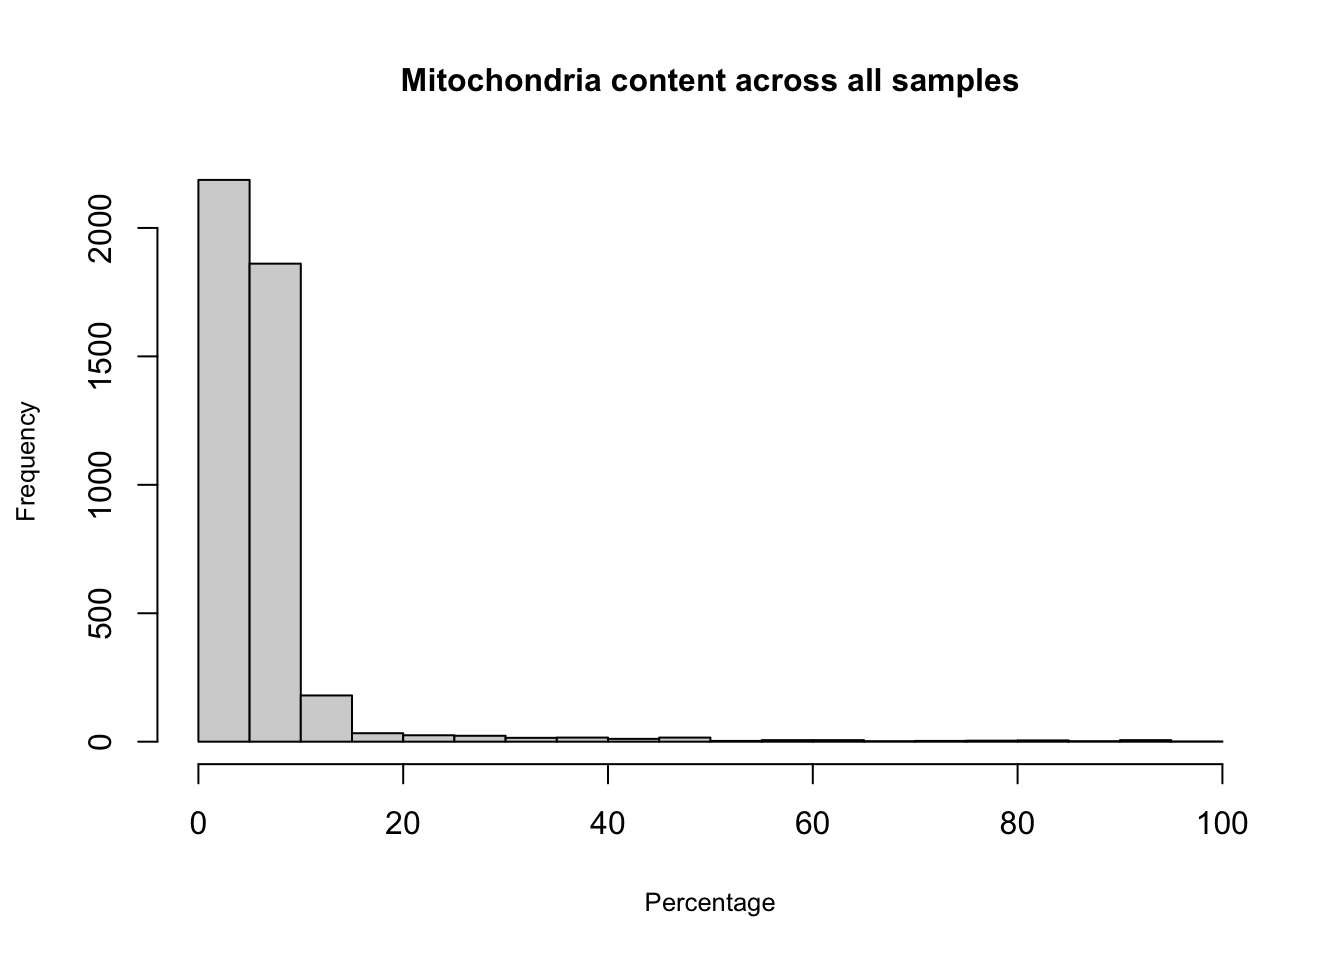
\includegraphics{scRNAseqtutorial_files/figure-latex/unnamed-chunk-18-1.pdf}
\caption{\label{fig:unnamed-chunk-18}Percentage of mitochondria}
\end{figure}

\begin{Shaded}
\begin{Highlighting}[]
\FunctionTok{par}\NormalTok{(}\AttributeTok{mfrow =} \FunctionTok{c}\NormalTok{(}\DecValTok{1}\NormalTok{,}\DecValTok{2}\NormalTok{), }\AttributeTok{oma =} \FunctionTok{c}\NormalTok{(}\DecValTok{0}\NormalTok{, }\DecValTok{0}\NormalTok{, }\DecValTok{4}\NormalTok{, }\DecValTok{0}\NormalTok{))}
\ControlFlowTok{for}\NormalTok{ (s }\ControlFlowTok{in}\NormalTok{ samples)}
\NormalTok{\{}
  \FunctionTok{hist}\NormalTok{(}
    \FunctionTok{subset}\NormalTok{(counts\_st}\SpecialCharTok{@}\NormalTok{meta.data, }\AttributeTok{subset =}\NormalTok{ Sample }\SpecialCharTok{==}\NormalTok{ s)}\SpecialCharTok{$}\NormalTok{percent.MT,}
    \AttributeTok{main =} \FunctionTok{paste0}\NormalTok{(s),}
    \AttributeTok{xlab =} \StringTok{"Percentage"}\NormalTok{,}
    \AttributeTok{cex.main =} \DecValTok{1}\NormalTok{,}
    \AttributeTok{cex.lab =} \FloatTok{0.9}\NormalTok{,}
    \AttributeTok{cex.axis =} \FloatTok{0.8}
\NormalTok{  )}
\NormalTok{\}}
\FunctionTok{title}\NormalTok{(}\AttributeTok{main =} \StringTok{"Mitochondria content"}\NormalTok{,}
      \AttributeTok{cex.main =} \DecValTok{1}\NormalTok{,}
      \AttributeTok{outer =}\NormalTok{ T)}
\end{Highlighting}
\end{Shaded}

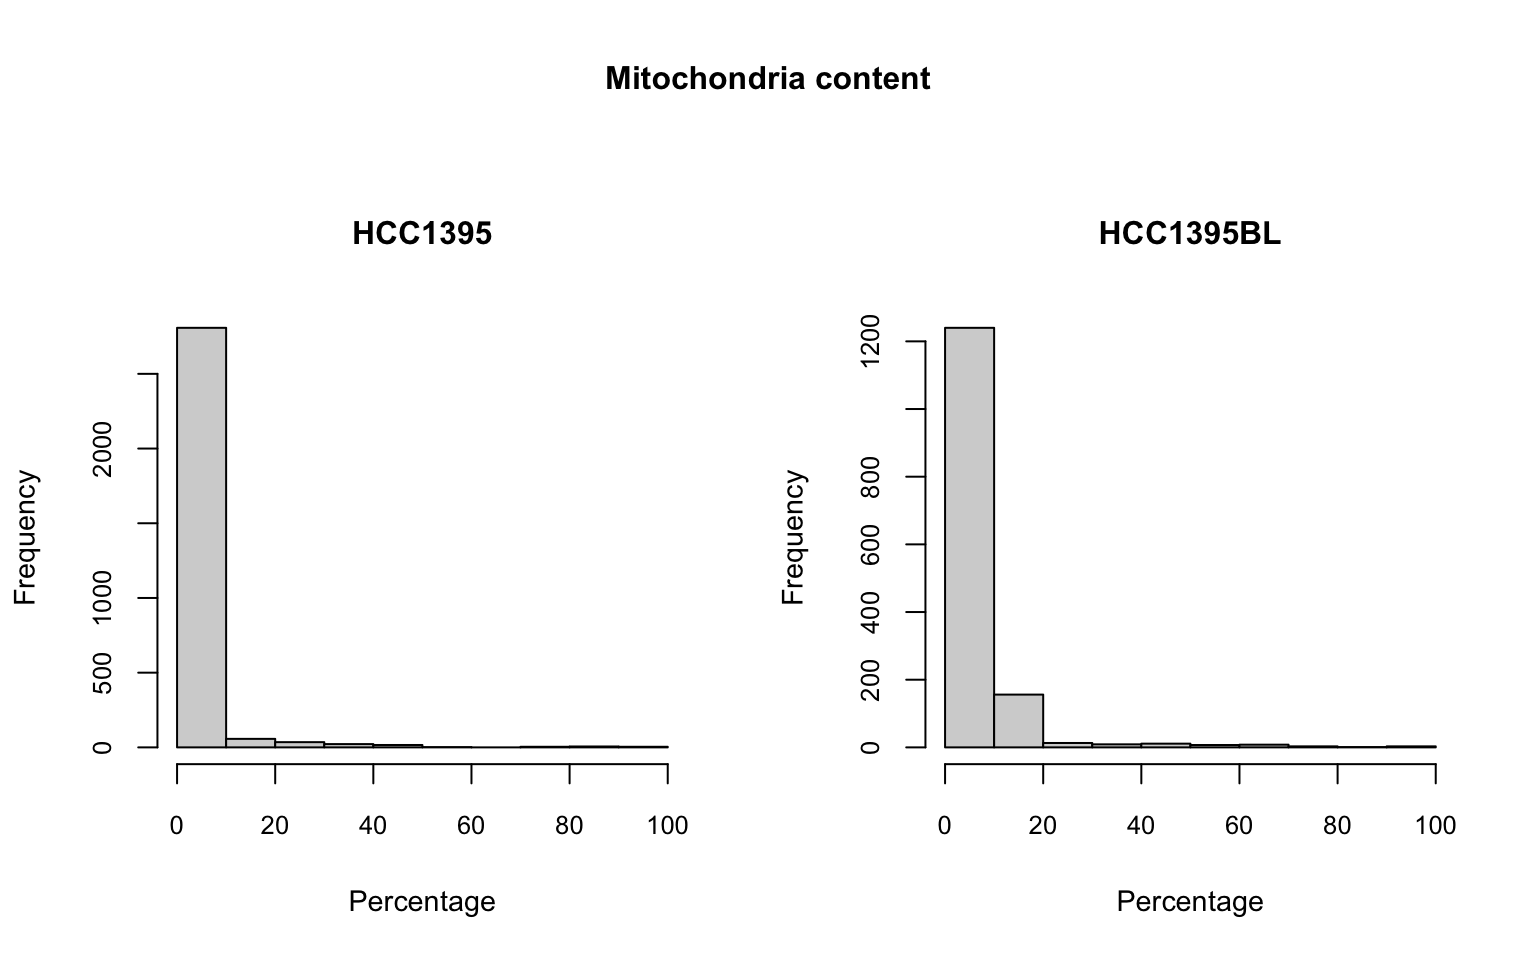
\includegraphics{scRNAseqtutorial_files/figure-latex/unnamed-chunk-19-1.pdf}

\hypertarget{ribosomal-content}{%
\subsection{Ribosomal content}\label{ribosomal-content}}

The histograms below show the distribution of the Ribosomal content across all samples.

\begin{Shaded}
\begin{Highlighting}[]
\FunctionTok{hist}\NormalTok{(}
\NormalTok{  counts\_st}\SpecialCharTok{@}\NormalTok{meta.data}\SpecialCharTok{$}\NormalTok{percent.Ribo,}
  \AttributeTok{xlab =} \StringTok{"Percentage"}\NormalTok{,}
  \AttributeTok{cex.main =} \DecValTok{1}\NormalTok{,}
  \AttributeTok{main =} \StringTok{"Ribosomal content across all samples"}\NormalTok{,}
  \AttributeTok{cex.lab =} \FloatTok{0.8}
\NormalTok{)}
\end{Highlighting}
\end{Shaded}

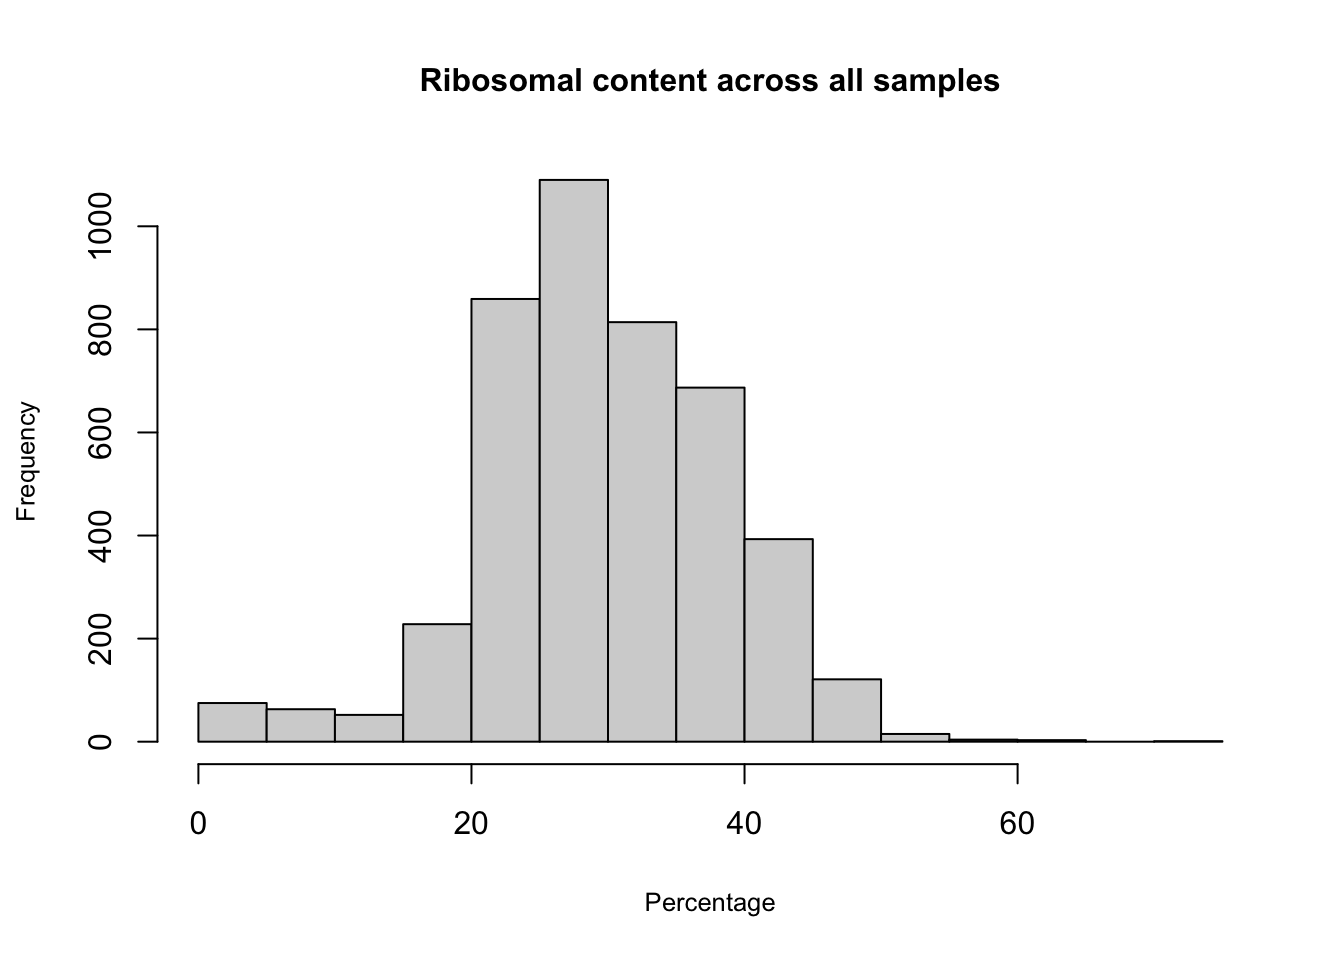
\includegraphics{scRNAseqtutorial_files/figure-latex/unnamed-chunk-20-1.pdf}

\begin{Shaded}
\begin{Highlighting}[]
\FunctionTok{par}\NormalTok{(}\AttributeTok{mfrow =} \FunctionTok{c}\NormalTok{(}\DecValTok{1}\NormalTok{, }\DecValTok{2}\NormalTok{), }\AttributeTok{oma =} \FunctionTok{c}\NormalTok{(}\DecValTok{0}\NormalTok{, }\DecValTok{0}\NormalTok{, }\DecValTok{4}\NormalTok{, }\DecValTok{0}\NormalTok{))}
\ControlFlowTok{for}\NormalTok{ (s }\ControlFlowTok{in}\NormalTok{ samples)}
\NormalTok{\{}
  \FunctionTok{hist}\NormalTok{(}
    \FunctionTok{subset}\NormalTok{(counts\_st}\SpecialCharTok{@}\NormalTok{meta.data, }\AttributeTok{subset =}\NormalTok{ Sample }\SpecialCharTok{==}\NormalTok{ s)}\SpecialCharTok{$}\NormalTok{percent.Ribo,}
    \AttributeTok{main =}\NormalTok{ s,}
    \AttributeTok{xlab =} \StringTok{"Percentage"}\NormalTok{,}
    \AttributeTok{cex.main =} \DecValTok{1}\NormalTok{,}
    \AttributeTok{cex.lab =} \FloatTok{0.9}\NormalTok{,}
    \AttributeTok{cex.axis =} \FloatTok{0.8}
\NormalTok{  )}
\NormalTok{\}}
\FunctionTok{title}\NormalTok{(}\AttributeTok{main =} \StringTok{"Ribosomal content"}\NormalTok{,}
      \AttributeTok{cex.main =} \DecValTok{1}\NormalTok{,}
      \AttributeTok{outer =}\NormalTok{ T)}
\end{Highlighting}
\end{Shaded}

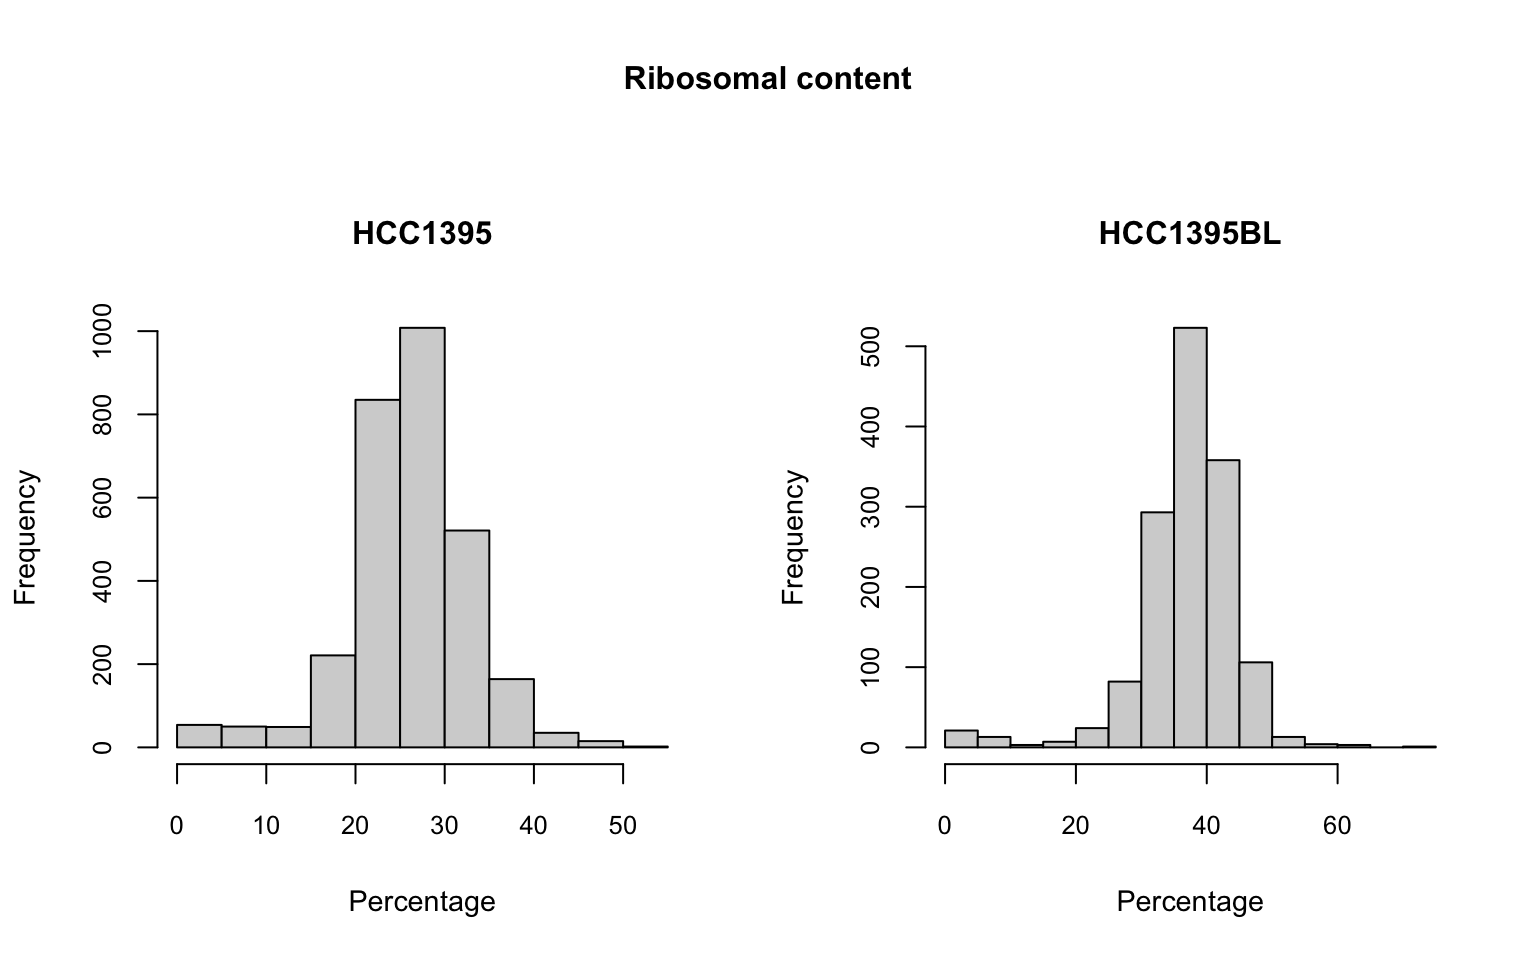
\includegraphics{scRNAseqtutorial_files/figure-latex/unnamed-chunk-21-1.pdf}

\hypertarget{number-of-detected-genes}{%
\subsection{Number of detected genes}\label{number-of-detected-genes}}

The histogram plot below shows the distribution of the number of detected genes across cells from all samples.

\begin{Shaded}
\begin{Highlighting}[]
\FunctionTok{hist}\NormalTok{(}
\NormalTok{  counts\_st}\SpecialCharTok{@}\NormalTok{meta.data}\SpecialCharTok{$}\NormalTok{nFeature\_RNA,}
  \AttributeTok{main =} \StringTok{"Number of detected genes "}\NormalTok{,}
  \AttributeTok{xlab =} \StringTok{"Genes per cell"}\NormalTok{,}
  \AttributeTok{cex.main =} \DecValTok{1}\NormalTok{,}
  \AttributeTok{cex.axis =} \FloatTok{0.9}\NormalTok{,}
  \AttributeTok{cex.lab =} \FloatTok{0.8}
\NormalTok{)}
\end{Highlighting}
\end{Shaded}

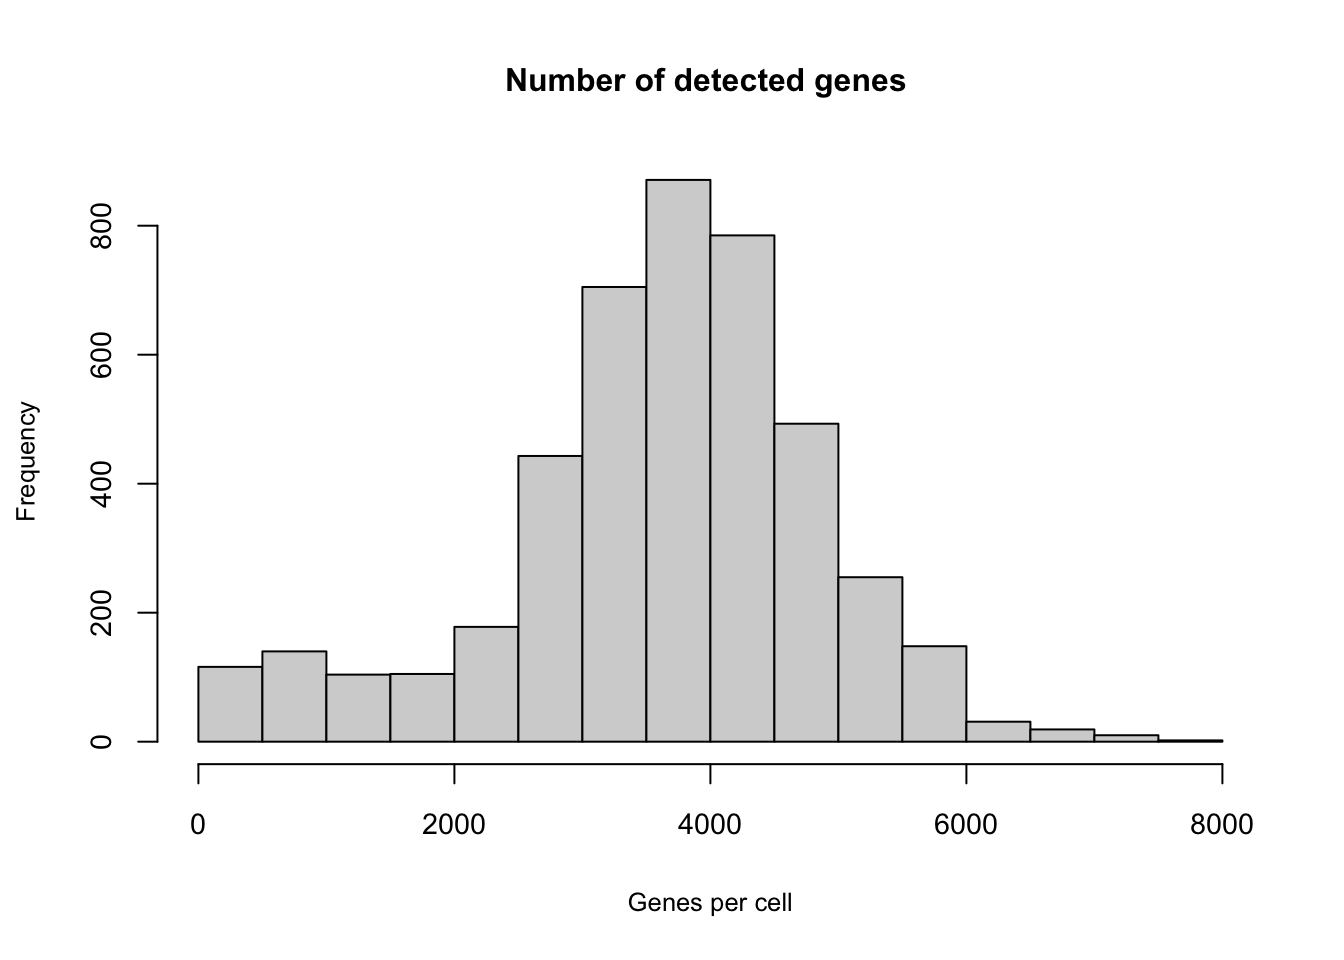
\includegraphics{scRNAseqtutorial_files/figure-latex/unnamed-chunk-22-1.pdf}

\begin{Shaded}
\begin{Highlighting}[]
\FunctionTok{par}\NormalTok{(}\AttributeTok{mfrow =} \FunctionTok{c}\NormalTok{(}\DecValTok{1}\NormalTok{, }\DecValTok{2}\NormalTok{), }\AttributeTok{oma =} \FunctionTok{c}\NormalTok{(}\DecValTok{0}\NormalTok{, }\DecValTok{0}\NormalTok{, }\DecValTok{4}\NormalTok{, }\DecValTok{0}\NormalTok{))}
\ControlFlowTok{for}\NormalTok{ (s }\ControlFlowTok{in}\NormalTok{ samples)}
\NormalTok{\{}
  \FunctionTok{hist}\NormalTok{(}
    \FunctionTok{subset}\NormalTok{(counts\_st}\SpecialCharTok{@}\NormalTok{meta.data, }\AttributeTok{subset =}\NormalTok{ Sample }\SpecialCharTok{==}\NormalTok{ s)}\SpecialCharTok{$}\NormalTok{nFeature\_RNA,}
    \AttributeTok{main =}\NormalTok{ s,}
    \AttributeTok{xlab =} \StringTok{"Detected genes"}\NormalTok{,}
    \AttributeTok{cex.main =} \DecValTok{1}\NormalTok{,}
    \AttributeTok{cex.lab =} \FloatTok{0.9}\NormalTok{,}
    \AttributeTok{cex.axis =} \FloatTok{0.8}
\NormalTok{  )}
\NormalTok{\}}
\FunctionTok{title}\NormalTok{(}\AttributeTok{main =} \StringTok{"Number of detected genes"}\NormalTok{,}
      \AttributeTok{outer =}\NormalTok{ T,}
      \AttributeTok{cex.main =} \DecValTok{1}\NormalTok{)}
\end{Highlighting}
\end{Shaded}

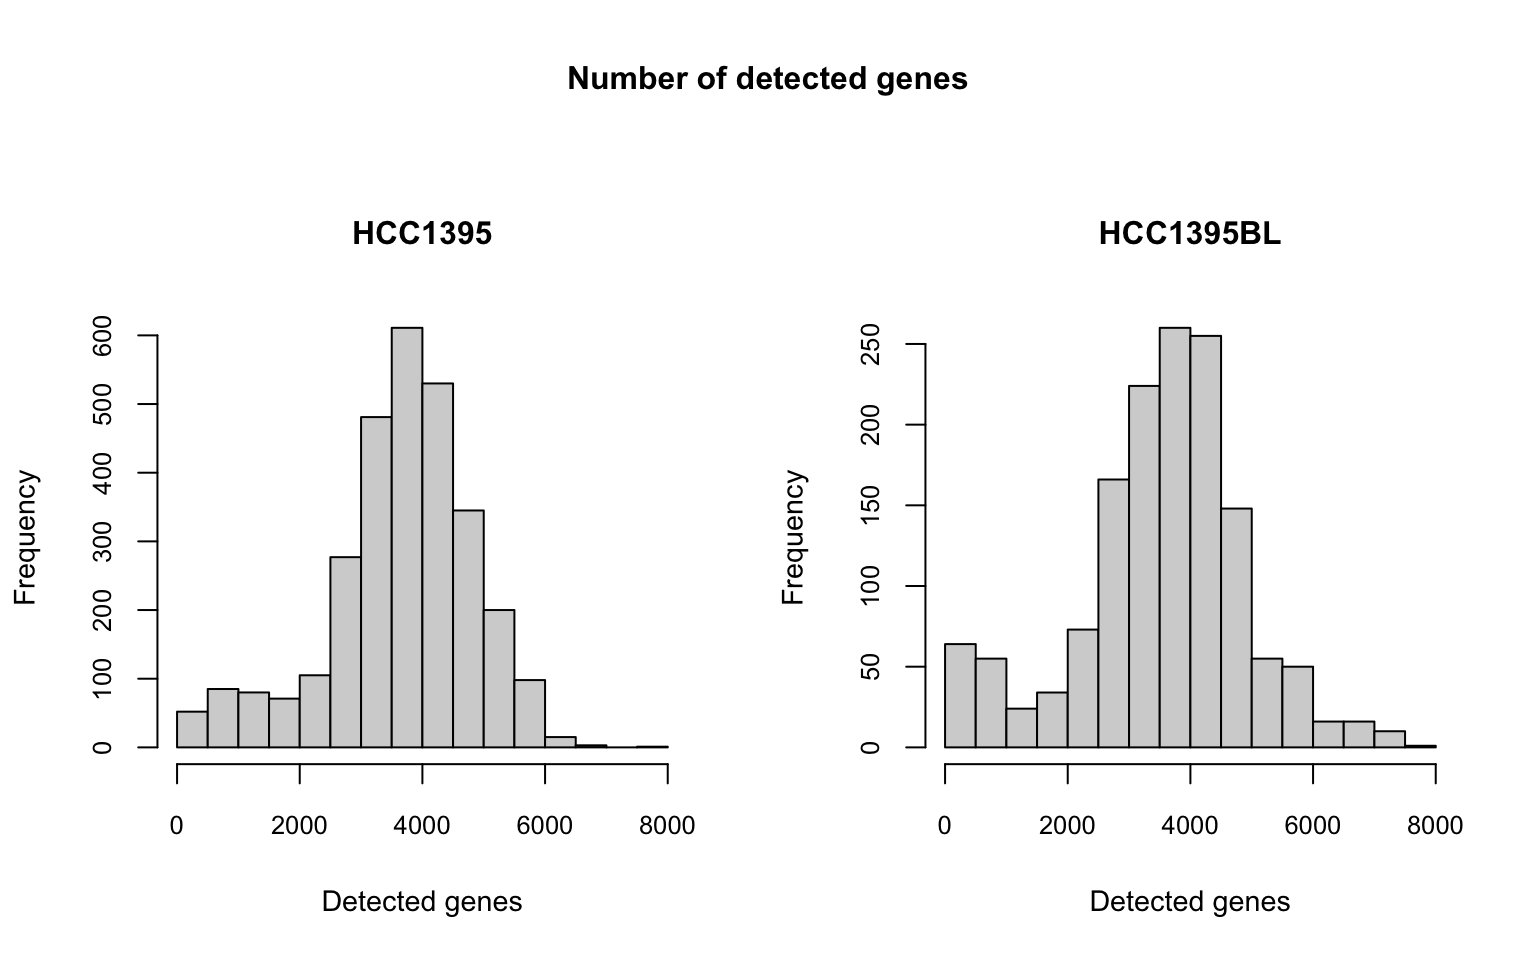
\includegraphics{scRNAseqtutorial_files/figure-latex/unnamed-chunk-23-1.pdf}

\hypertarget{filtering}{%
\section{Filtering}\label{filtering}}

\hypertarget{cell-filtering}{%
\subsection{Cell filtering}\label{cell-filtering}}

\begin{Shaded}
\begin{Highlighting}[]
\CommentTok{\#Filters used }
\NormalTok{min.exp\_genes}\OtherTok{\textless{}{-}}\DecValTok{200} \CommentTok{\#minimum number of detected genes in each cell}
\NormalTok{max.exp\_genes}\OtherTok{\textless{}{-}}\DecValTok{6000} \CommentTok{\#Maximum number of detected genes in each cell}
\NormalTok{percent.mito }\OtherTok{\textless{}{-}} \DecValTok{20} \CommentTok{\#Percentage of mitochondrial content}
\NormalTok{percent.ribos }\OtherTok{\textless{}{-}} \DecValTok{40} \CommentTok{\# Max percentage of Ribosomal content}
\end{Highlighting}
\end{Shaded}

Based on the quality control checks above, the following filters are used to exclude cells that did not meet the criteria from the rest of the analysis

\begin{itemize}
\item cells with <200 detected genes
\item cells with >6000 detected genes
\item cells with >20 of Mitochondria content per cell
\item cells with > 40 of Ribosomal content per cell
\end{itemize}

Number of cells before filtering for mitochondrial and ribosomal content: 4,405

\begin{Shaded}
\begin{Highlighting}[]
\CommentTok{\#exclude cells with a high content of mitochondrial and ribosomal content}
\NormalTok{counts\_st }\OtherTok{\textless{}{-}}\FunctionTok{subset}\NormalTok{(counts\_st, }\AttributeTok{subset =}\NormalTok{ percent.MT }\SpecialCharTok{\textless{}}\NormalTok{ percent.mito }\SpecialCharTok{\&}
\NormalTok{           percent.Ribo }\SpecialCharTok{\textless{}}\NormalTok{ percent.ribos)}
\end{Highlighting}
\end{Shaded}

Number of cells after filtering for mitochondria and ribosomal content: 3,731
Next we exclude cells that had less than 200 and greater than 6,000

\begin{Shaded}
\begin{Highlighting}[]
\CommentTok{\#exclude cells with low or high number of detected features}
\NormalTok{counts\_st }\OtherTok{\textless{}{-}}\FunctionTok{subset}\NormalTok{(counts\_st,}\AttributeTok{subset =}\NormalTok{ nFeature\_RNA }\SpecialCharTok{\textgreater{}=}\NormalTok{ min.exp\_genes }\SpecialCharTok{\&}\NormalTok{ nFeature\_RNA }\SpecialCharTok{\textless{}=}\NormalTok{ max.exp\_genes)}
\end{Highlighting}
\end{Shaded}

Number of cells remaining after filtering for cells with
low number of detected genes: 3,678
Number of cells left per sample

HCC1395 HCC1395BL
2794 884

\hypertarget{gene-filtering}{%
\subsection{Gene filtering}\label{gene-filtering}}

Genes that failed to express (an expressed gene has at least 1 UMI count) in at least 3 cells in at least 1 sample together with Mitochondrial and Ribosomal genes are excluded from the rest of the analysis;

Number of genes before filter: 28,395

\begin{Shaded}
\begin{Highlighting}[]
\CommentTok{\#Check genes expressed in at least 3 cells in at least one of the samples}
\NormalTok{keep.genes }\OtherTok{\textless{}{-}} \FunctionTok{rowSums}\NormalTok{(}\FunctionTok{do.call}\NormalTok{(cbind, }\FunctionTok{lapply}\NormalTok{(samples, }\ControlFlowTok{function}\NormalTok{(x)}
  \FunctionTok{rowSums}\NormalTok{(}\FunctionTok{subset}\NormalTok{(counts\_st, Sample }\SpecialCharTok{==}\NormalTok{ x)}\SpecialCharTok{@}\NormalTok{assays}\SpecialCharTok{$}\NormalTok{RNA}\SpecialCharTok{@}\NormalTok{counts }\SpecialCharTok{\textgreater{}} \DecValTok{0}\NormalTok{) }\SpecialCharTok{\textgreater{}=} \DecValTok{3}\NormalTok{))) }\SpecialCharTok{\textgreater{}}
  \DecValTok{0}
\FunctionTok{table}\NormalTok{(keep.genes)}
\end{Highlighting}
\end{Shaded}

\begin{verbatim}
## keep.genes
## FALSE  TRUE 
## 10516 17879
\end{verbatim}

\begin{Shaded}
\begin{Highlighting}[]
\NormalTok{counts\_st }\OtherTok{\textless{}{-}}\NormalTok{ counts\_st[keep.genes, ]}
\end{Highlighting}
\end{Shaded}

Number of genes after filtering for genes that failed to express in at least 3 cells in at least 1 sample: 17,879

Mitochondrial and Ribosomal genes are also excluded from the rest of the analysis.

\begin{Shaded}
\begin{Highlighting}[]
\CommentTok{\#filter ribosomal and mitochondrial genes}
\NormalTok{counts\_st }\OtherTok{\textless{}{-}}
\NormalTok{  counts\_st[}\SpecialCharTok{!}\NormalTok{(}\FunctionTok{rownames}\NormalTok{(counts\_st) }\SpecialCharTok{\%in\%}\NormalTok{ genes.MT) }\SpecialCharTok{\&}
       \SpecialCharTok{!}\FunctionTok{grepl}\NormalTok{(}\StringTok{"\^{}RP[SL]"}\NormalTok{, }\FunctionTok{rownames}\NormalTok{(counts\_st)),]}
\end{Highlighting}
\end{Shaded}

Number of genes after filtering for mitochondrial and ribosomal genes: 17,711

\hypertarget{normalization}{%
\section{Normalization}\label{normalization}}

After removing unwanted cells from the dataset, the data was normalized using a global-scaling normalization method ``LogNormalize'' that normalizes the feature expression measurements for each cell by the total expression, multiplies this by a scale factor (10,000 by default), and log-transforms the result.

\begin{Shaded}
\begin{Highlighting}[]
\NormalTok{counts\_st }\OtherTok{\textless{}{-}}\FunctionTok{NormalizeData}\NormalTok{(}
    \AttributeTok{object =}\NormalTok{ counts\_st,}
    \AttributeTok{normalization.method =} \StringTok{"LogNormalize"}\NormalTok{,}
    \AttributeTok{scale.factor =} \DecValTok{10000}
\NormalTok{  )}
\end{Highlighting}
\end{Shaded}

\hypertarget{dimension-reduction-and-clustering}{%
\section{Dimension reduction and clustering}\label{dimension-reduction-and-clustering}}

A subset of highly variable genes between cells were calculated using \emph{FindVariableFeatures} function within Seurat.

\begin{Shaded}
\begin{Highlighting}[]
\CommentTok{\#Identification of highly variable features (feature selection)}
\NormalTok{counts\_st }\OtherTok{\textless{}{-}} \FunctionTok{FindVariableFeatures}\NormalTok{(}\AttributeTok{object =}\NormalTok{ counts\_st )}
\end{Highlighting}
\end{Shaded}

The scatter plot below shows the top 10 identified variable genes and their average expression against variance

\begin{Shaded}
\begin{Highlighting}[]
\CommentTok{\# Identify the 10 most highly variable genes}
\NormalTok{top10 }\OtherTok{\textless{}{-}} \FunctionTok{head}\NormalTok{(}\FunctionTok{VariableFeatures}\NormalTok{(counts\_st), }\DecValTok{10}\NormalTok{)}
\CommentTok{\# plot variable features with labels}
\NormalTok{plot1 }\OtherTok{\textless{}{-}} \FunctionTok{VariableFeaturePlot}\NormalTok{(counts\_st)}
\NormalTok{plot2 }\OtherTok{\textless{}{-}} \FunctionTok{LabelPoints}\NormalTok{(}\AttributeTok{plot =}\NormalTok{ plot1, }\AttributeTok{points =}\NormalTok{ top10, }\AttributeTok{repel =} \ConstantTok{TRUE}\NormalTok{)}
\end{Highlighting}
\end{Shaded}

\begin{verbatim}
## When using repel, set xnudge and ynudge to 0 for optimal results
\end{verbatim}

\begin{Shaded}
\begin{Highlighting}[]
\NormalTok{plot2}
\end{Highlighting}
\end{Shaded}

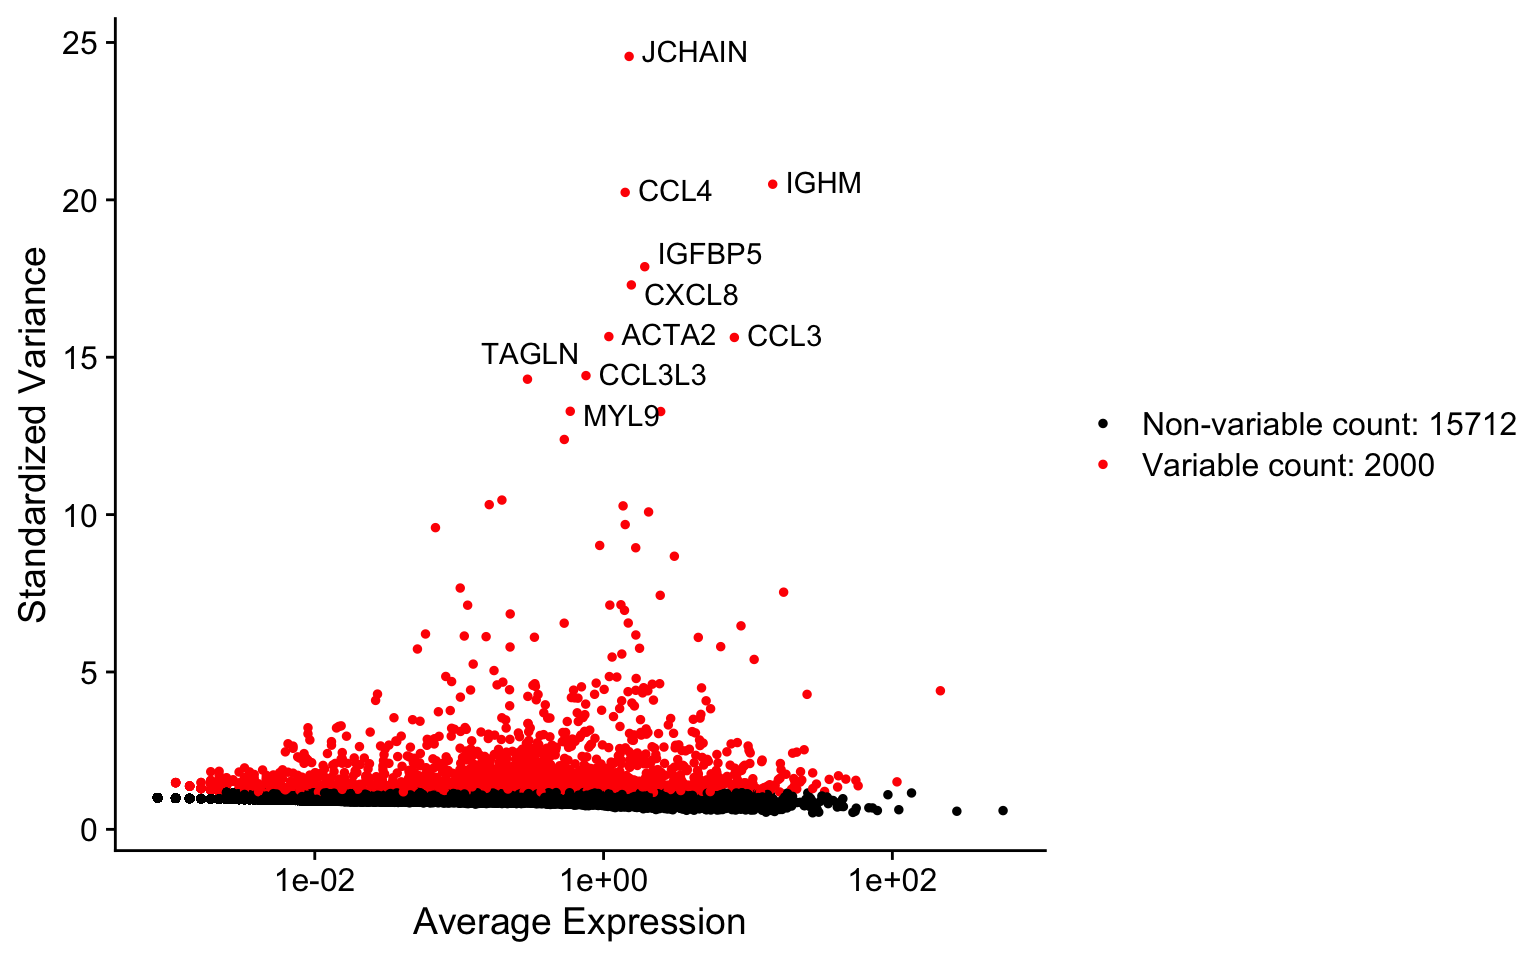
\includegraphics{scRNAseqtutorial_files/figure-latex/unnamed-chunk-37-1.pdf}

A linear transformation (`scaling') was applied to the normalized data prior to dimensional reduction techniques using the \emph{ScaleData} function in \textbf{Seurat}.

\begin{Shaded}
\begin{Highlighting}[]
\NormalTok{counts\_st }\OtherTok{\textless{}{-}}  \FunctionTok{ScaleData}\NormalTok{(}
    \AttributeTok{object =}\NormalTok{ counts\_st,}
    \AttributeTok{features =} \FunctionTok{rownames}\NormalTok{(counts\_st),}
    \AttributeTok{verbose =}\NormalTok{ F)}
\end{Highlighting}
\end{Shaded}

Principal component analysis was performed using the variable genes identified above.

\begin{Shaded}
\begin{Highlighting}[]
\NormalTok{counts\_st }\OtherTok{\textless{}{-}}\FunctionTok{RunPCA}\NormalTok{(}
\NormalTok{    counts\_st,}
    \AttributeTok{features =} \FunctionTok{VariableFeatures}\NormalTok{(}\AttributeTok{object =}\NormalTok{ counts\_st))}
\end{Highlighting}
\end{Shaded}

\begin{verbatim}
## PC_ 1 
## Positive:  S100A6, S100A10, TNFRSF12A, TSPO, TPM2, CAV1, TPM1, CALD1, ANXA2, RHEB 
##     ITGB1, LARP6, NQO1, HSBP1, SERPINE2, MGST1, FTH1P3, HSPB1, CYP1B1, KRT81 
##     DEF8, TSC22D1, LY6K, TNNT1, TGFBI, CAV2, CALU, DSTN, CCND1, TUBB3 
## Negative:  CD74, HLA-DRA, MS4A1, HLA-DPA1, LAPTM5, ARHGDIB, HLA-DPB1, IGHM, LSP1, LIMD2 
##     MIR155HG, CD70, CCND2, PDLIM1, CORO1A, BST2, CD79A, SNCA, CCL3, CD48 
##     RAC2, SRGN, TMSB4X, IGLC2, PLEK, CCR7, HCLS1, TNFRSF13B, CD53, IRF4 
## PC_ 2 
## Positive:  NME7, NDRG1, GADD45A, WIPI1, YPEL5, H2BC12, LURAP1L, GABARAPL1, GDF5, ZNF667-AS1 
##     ULK4, MYLK, KRT16, CCN1, FN1, LINC01315, NUPR1, BEX2, DNAJB9, PLK2 
##     SGK1, KRT75, CCN2, FBLIM1, MYC, MAP1LC3B, SELENOM, LINC01133, DUSP10, IL1RL1 
## Negative:  MKI67, CENPF, PLK1, HMGB2, CDC20, AURKA, CDCA3, UBE2C, CENPA, CCNA2 
##     GTSE1, HMMR, PTTG1, TPX2, NUSAP1, SMC4, TOP2A, CKS2, CENPE, CCNB1 
##     CDKN3, BIRC5, PRC1, CCNB2, ARL6IP1, DEPDC1, SGO2, ASPM, UBE2S, KPNA2 
## PC_ 3 
## Positive:  ULK4, ASPM, MKI67, C1orf56, CENPF, JCHAIN, TOP2A, GTSE1, NUSAP1, MXD3 
##     HMGB2, CDKN3, KIF14, CENPA, IGLL1, HMMR, IGLC7, BIRC5, PHKG1, IGLC5 
##     ITGA4, PRDM1, CENPE, CKAP2, TPX2, PRR11, DLGAP5, CDCA3, PIF1, IGLL5 
## Negative:  GADD45A, MARCKSL1, LAPTM4A, FDPS, ATP6V0B, PSMD8, PSMC2, HLA-C, PRMT1, TAGLN2 
##     CD44, TMBIM6, PAK1IP1, LGMN, DNAJA1, UBB, XRCC6, ENO1, TIMP1, RIPK2 
##     HACD3, DCAF13, UBC, TXNL1, HCCS, ADH5, CCT4, RTCB, DNAJB6, PGK1 
## PC_ 4 
## Positive:  ZFP36L1, DEK, BASP1, H4C3, STAG3, C12orf75, CCL22, SCG5, SERTAD4-AS1, CD82 
##     ATAD2, TNFSF4, CENPX, PRRX1, ARL4C, HCFC1R1, TNFAIP3, RAC3, FAM20C, DUSP4 
##     GTSE1, FTH1P3, ANKRD33B, SOX4, MARCKSL1, TNNT1, ANKRD11, PRR11, SMIM14, RUNX3 
## Negative:  UBB, PRDX1, PGK1, PSMA4, ENO1, PSMA3, EIF4A3, TMBIM6, ERP44, JCHAIN 
##     DCAF13, NPM1, CCT8, XRCC6, PSME2, IGLL1, IGLC7, IGLC5, MDH1, HSPA5 
##     HSPD1, HSP90AB1, CCT4, CCT5, HSP90B1, PSMC2, UBC, IGLL5, PRMT1, DNAJB11 
## PC_ 5 
## Positive:  C12orf75, JCHAIN, IGLC7, IGLL1, IGLC5, IGLL5, FN1, FTL, ITGA4, SPHK1 
##     PRDM1, TNFRSF17, GLCCI1, SSR3, IGLL3P, RASSF6, GUSBP11, LINC01480, CLEC2B, ST6GAL1 
##     GLIPR1, ISG15, XBP1, POU2AF1, FAM107B, SDF2L1, RRAGD, CCDC69, MEF2C, CYTOR 
## Negative:  MMP7, LTA, AKR1C2, WDR91, BCL2A1, CCL22, AKR1C1, PRDX1, ENO1, SSTR2 
##     HSP90AB1, LDHA, AKR1C3, TRAF1, TNFRSF8, STAG3, PKM, HSPD1, EBI3, AKR1B10 
##     MUC12-AS1, LINC00158, ICAM1, HSP90AA1, ZBTB32, RHOV, AKR1C4, NFKBIA, CCT5, BCAT1
\end{verbatim}

We use the \emph{JackStraw} function in \textbf{Seurat} to establish the dimensionality of the dataset. This is done by randomly selecting a subset of genes and their significance in a computed PC.

\begin{Shaded}
\begin{Highlighting}[]
\NormalTok{counts\_st }\OtherTok{\textless{}{-}} \FunctionTok{JackStraw}\NormalTok{(counts\_st, }\AttributeTok{verbose =}\NormalTok{ F, }\AttributeTok{dims =} \DecValTok{20}\NormalTok{)}
\NormalTok{counts\_st }\OtherTok{\textless{}{-}}
  \FunctionTok{ScoreJackStraw}\NormalTok{(counts\_st, }\AttributeTok{reduction =} \StringTok{"pca"}\NormalTok{, }\AttributeTok{dims =} \DecValTok{1}\SpecialCharTok{:}\DecValTok{20}\NormalTok{)}
\end{Highlighting}
\end{Shaded}

\begin{Shaded}
\begin{Highlighting}[]
\FunctionTok{JackStrawPlot}\NormalTok{(counts\_st, }\AttributeTok{reduction =} \StringTok{"pca"}\NormalTok{, }\AttributeTok{dims =} \DecValTok{1}\SpecialCharTok{:}\DecValTok{20}\NormalTok{)}
\end{Highlighting}
\end{Shaded}

\begin{verbatim}
## Warning: Removed 28000 rows containing missing values (geom_point).
\end{verbatim}

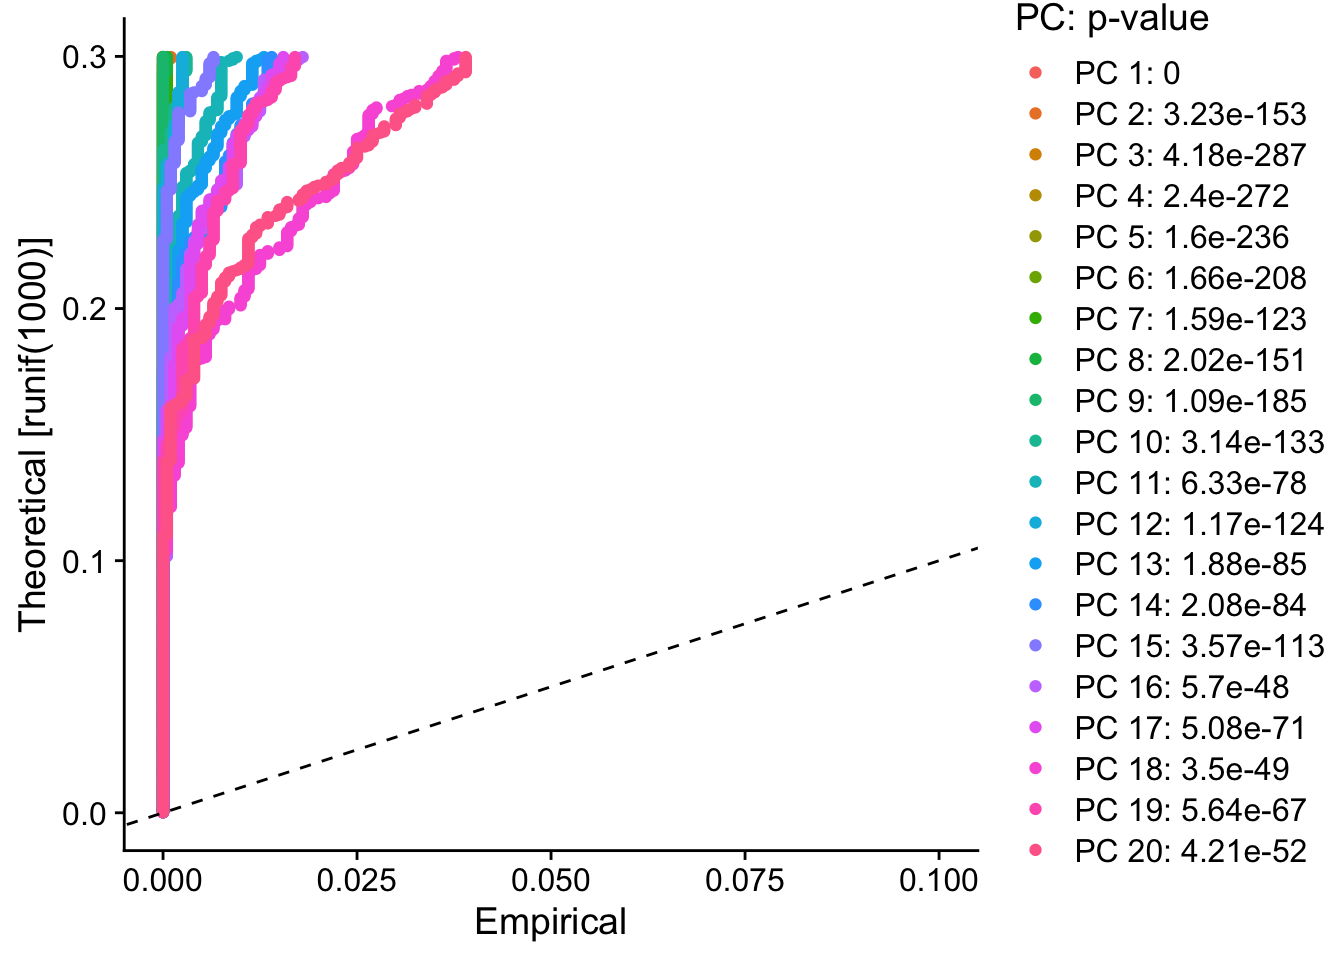
\includegraphics{scRNAseqtutorial_files/figure-latex/elbowplot1-1.pdf}

\begin{Shaded}
\begin{Highlighting}[]
\FunctionTok{ElbowPlot}\NormalTok{(counts\_st)}
\end{Highlighting}
\end{Shaded}

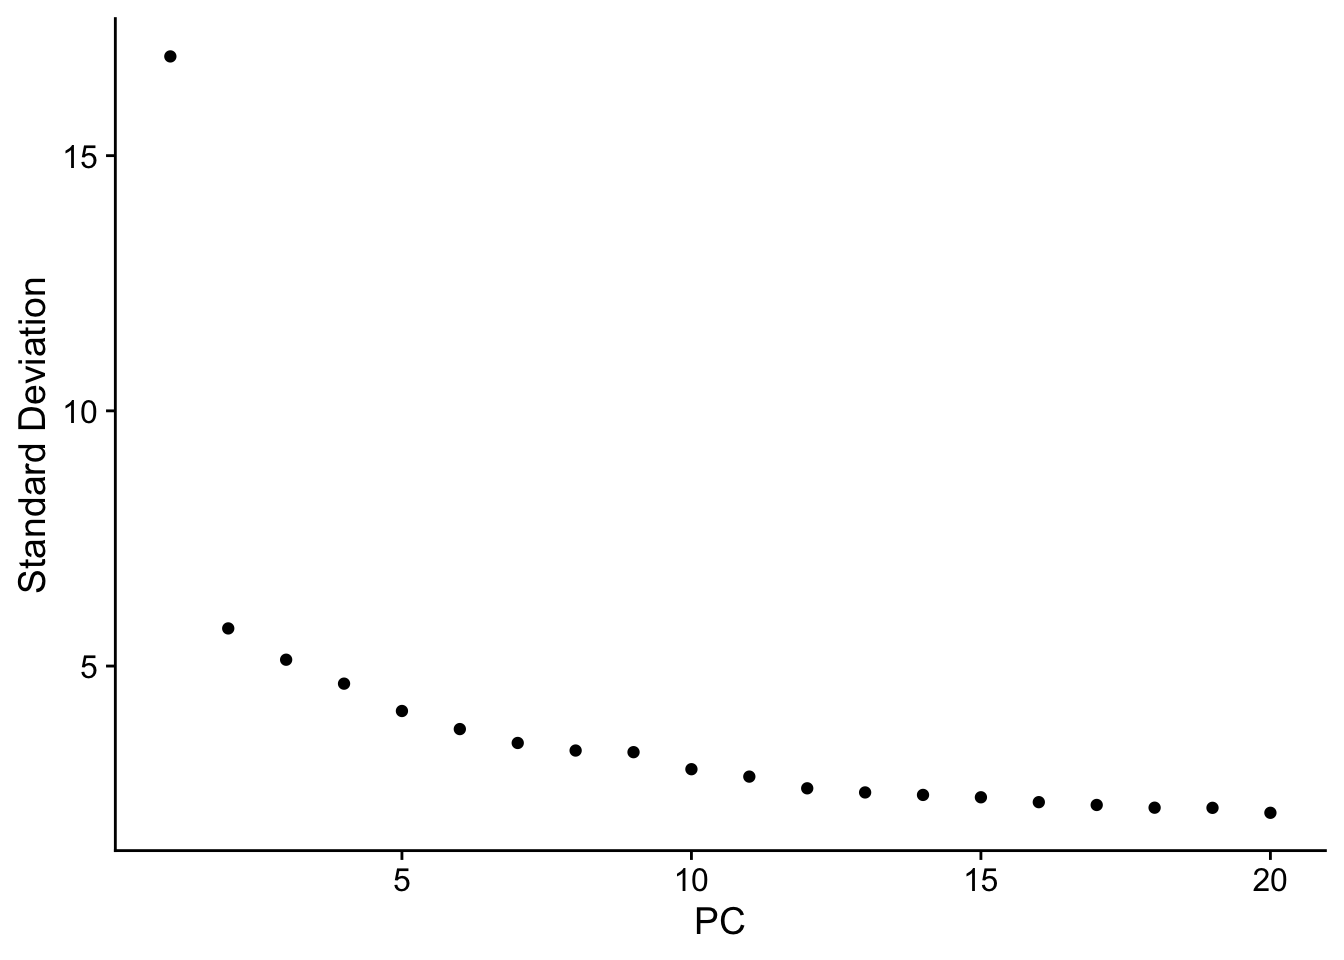
\includegraphics{scRNAseqtutorial_files/figure-latex/elbowplot1-2.pdf}

\begin{Shaded}
\begin{Highlighting}[]
\NormalTok{res}\OtherTok{\textless{}{-}}\FloatTok{0.5}
\NormalTok{sel.dims}\OtherTok{\textless{}{-}}\DecValTok{10}
\end{Highlighting}
\end{Shaded}

10 dimensions are used to establish the number of clusters with a resolution of 0.5

\begin{Shaded}
\begin{Highlighting}[]
\NormalTok{counts\_st }\OtherTok{\textless{}{-}}\FunctionTok{FindNeighbors}\NormalTok{(counts\_st,}
                \AttributeTok{reduction =} \StringTok{"pca"}\NormalTok{,}
                \AttributeTok{verbose =}\NormalTok{ F,}
                \AttributeTok{dims =} \DecValTok{1}\SpecialCharTok{:}\NormalTok{sel.dims)}
\end{Highlighting}
\end{Shaded}

Next we run the \textbf{FindClusters} to identify clusters of cells using a resolution of 0.5.

\begin{Shaded}
\begin{Highlighting}[]
\NormalTok{counts\_st }\OtherTok{\textless{}{-}}
  \FunctionTok{FindClusters}\NormalTok{(}
    \AttributeTok{object =}\NormalTok{ counts\_st,}
    \AttributeTok{resolution =}\NormalTok{ res,}
    \AttributeTok{verbose =} \DecValTok{0}
\NormalTok{  )}
\end{Highlighting}
\end{Shaded}

t-SNE dimensionality reduction on is run on the identified variable features.

\begin{Shaded}
\begin{Highlighting}[]
\NormalTok{counts\_st }\OtherTok{\textless{}{-}} \FunctionTok{RunTSNE}\NormalTok{(counts\_st, }\AttributeTok{dims =} \DecValTok{1}\SpecialCharTok{:}\NormalTok{sel.dims)}
\end{Highlighting}
\end{Shaded}

\begin{Shaded}
\begin{Highlighting}[]
\FunctionTok{DimPlot}\NormalTok{(}
\NormalTok{  counts\_st,}
  \AttributeTok{reduction =} \StringTok{"tsne"}\NormalTok{,}
  \AttributeTok{label =}\NormalTok{ T,}
  \AttributeTok{size =} \FloatTok{0.5}\NormalTok{,}
  \AttributeTok{repel =}\NormalTok{ T,}
  \AttributeTok{cols =} \FunctionTok{DiscretePalette}\NormalTok{(}\FunctionTok{length}\NormalTok{(}\FunctionTok{levels}\NormalTok{(}\FunctionTok{Idents}\NormalTok{(}
\NormalTok{    counts\_st}
\NormalTok{  ))))}
\NormalTok{)}
\end{Highlighting}
\end{Shaded}

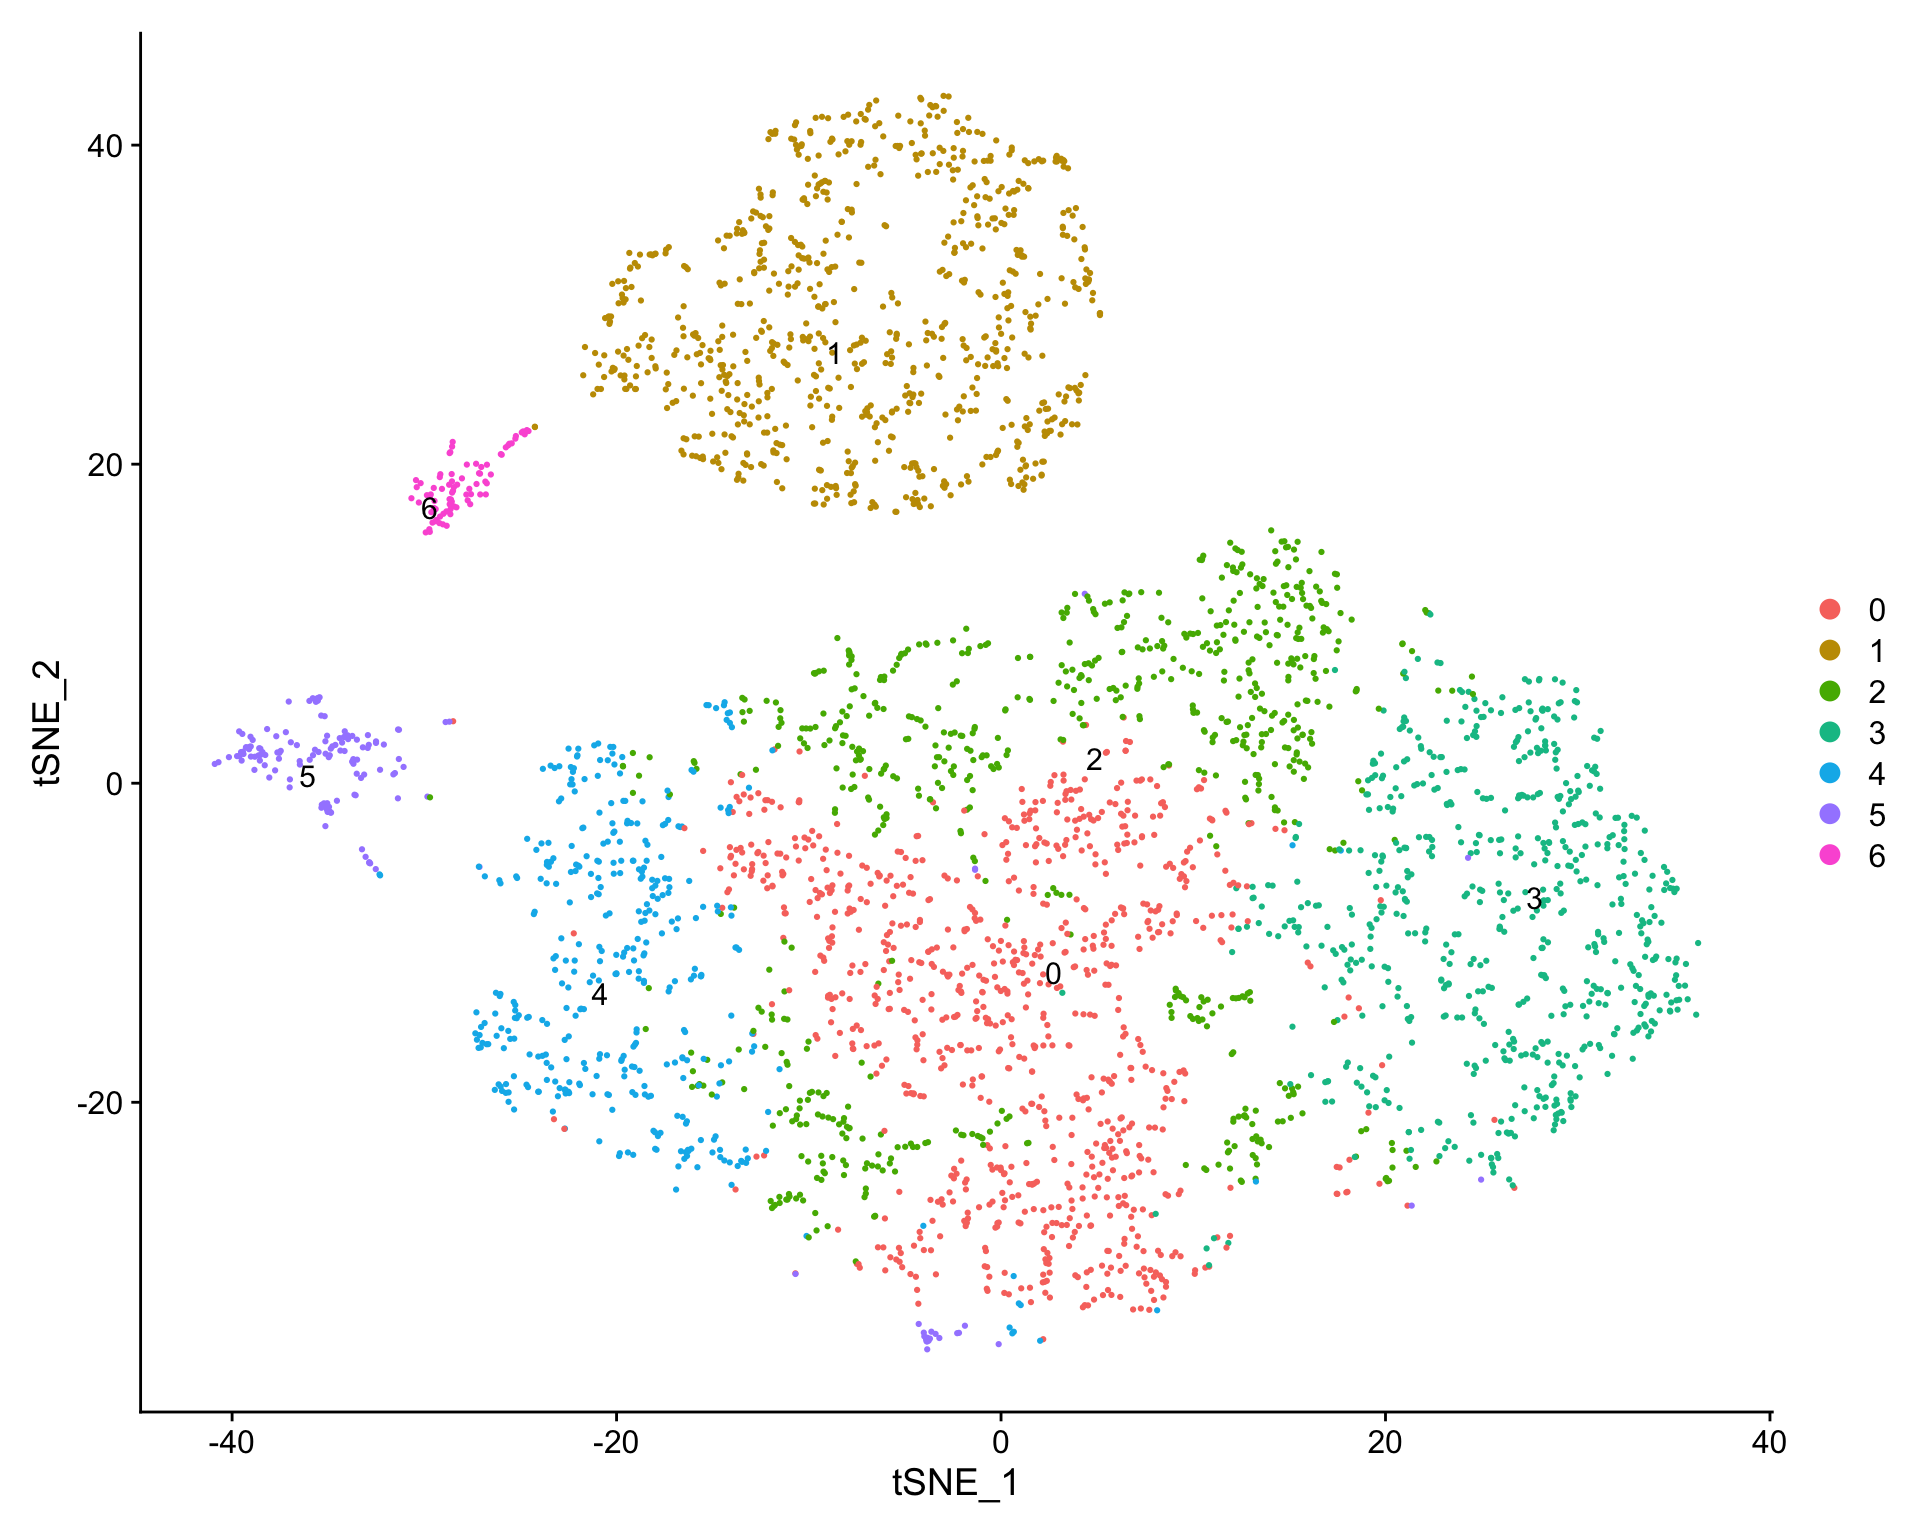
\includegraphics{scRNAseqtutorial_files/figure-latex/unnamed-chunk-42-1.pdf}

\begin{Shaded}
\begin{Highlighting}[]
\FunctionTok{DimPlot}\NormalTok{(}
\NormalTok{  counts\_st,}
  \AttributeTok{reduction =} \StringTok{"tsne"}\NormalTok{,}
  \AttributeTok{label =}\NormalTok{ T,}
  \AttributeTok{group.by =} \StringTok{"Sample"}\NormalTok{,}
  \AttributeTok{size =} \FloatTok{0.5}\NormalTok{,}
  \AttributeTok{repel =}\NormalTok{ T}
\NormalTok{)}
\end{Highlighting}
\end{Shaded}

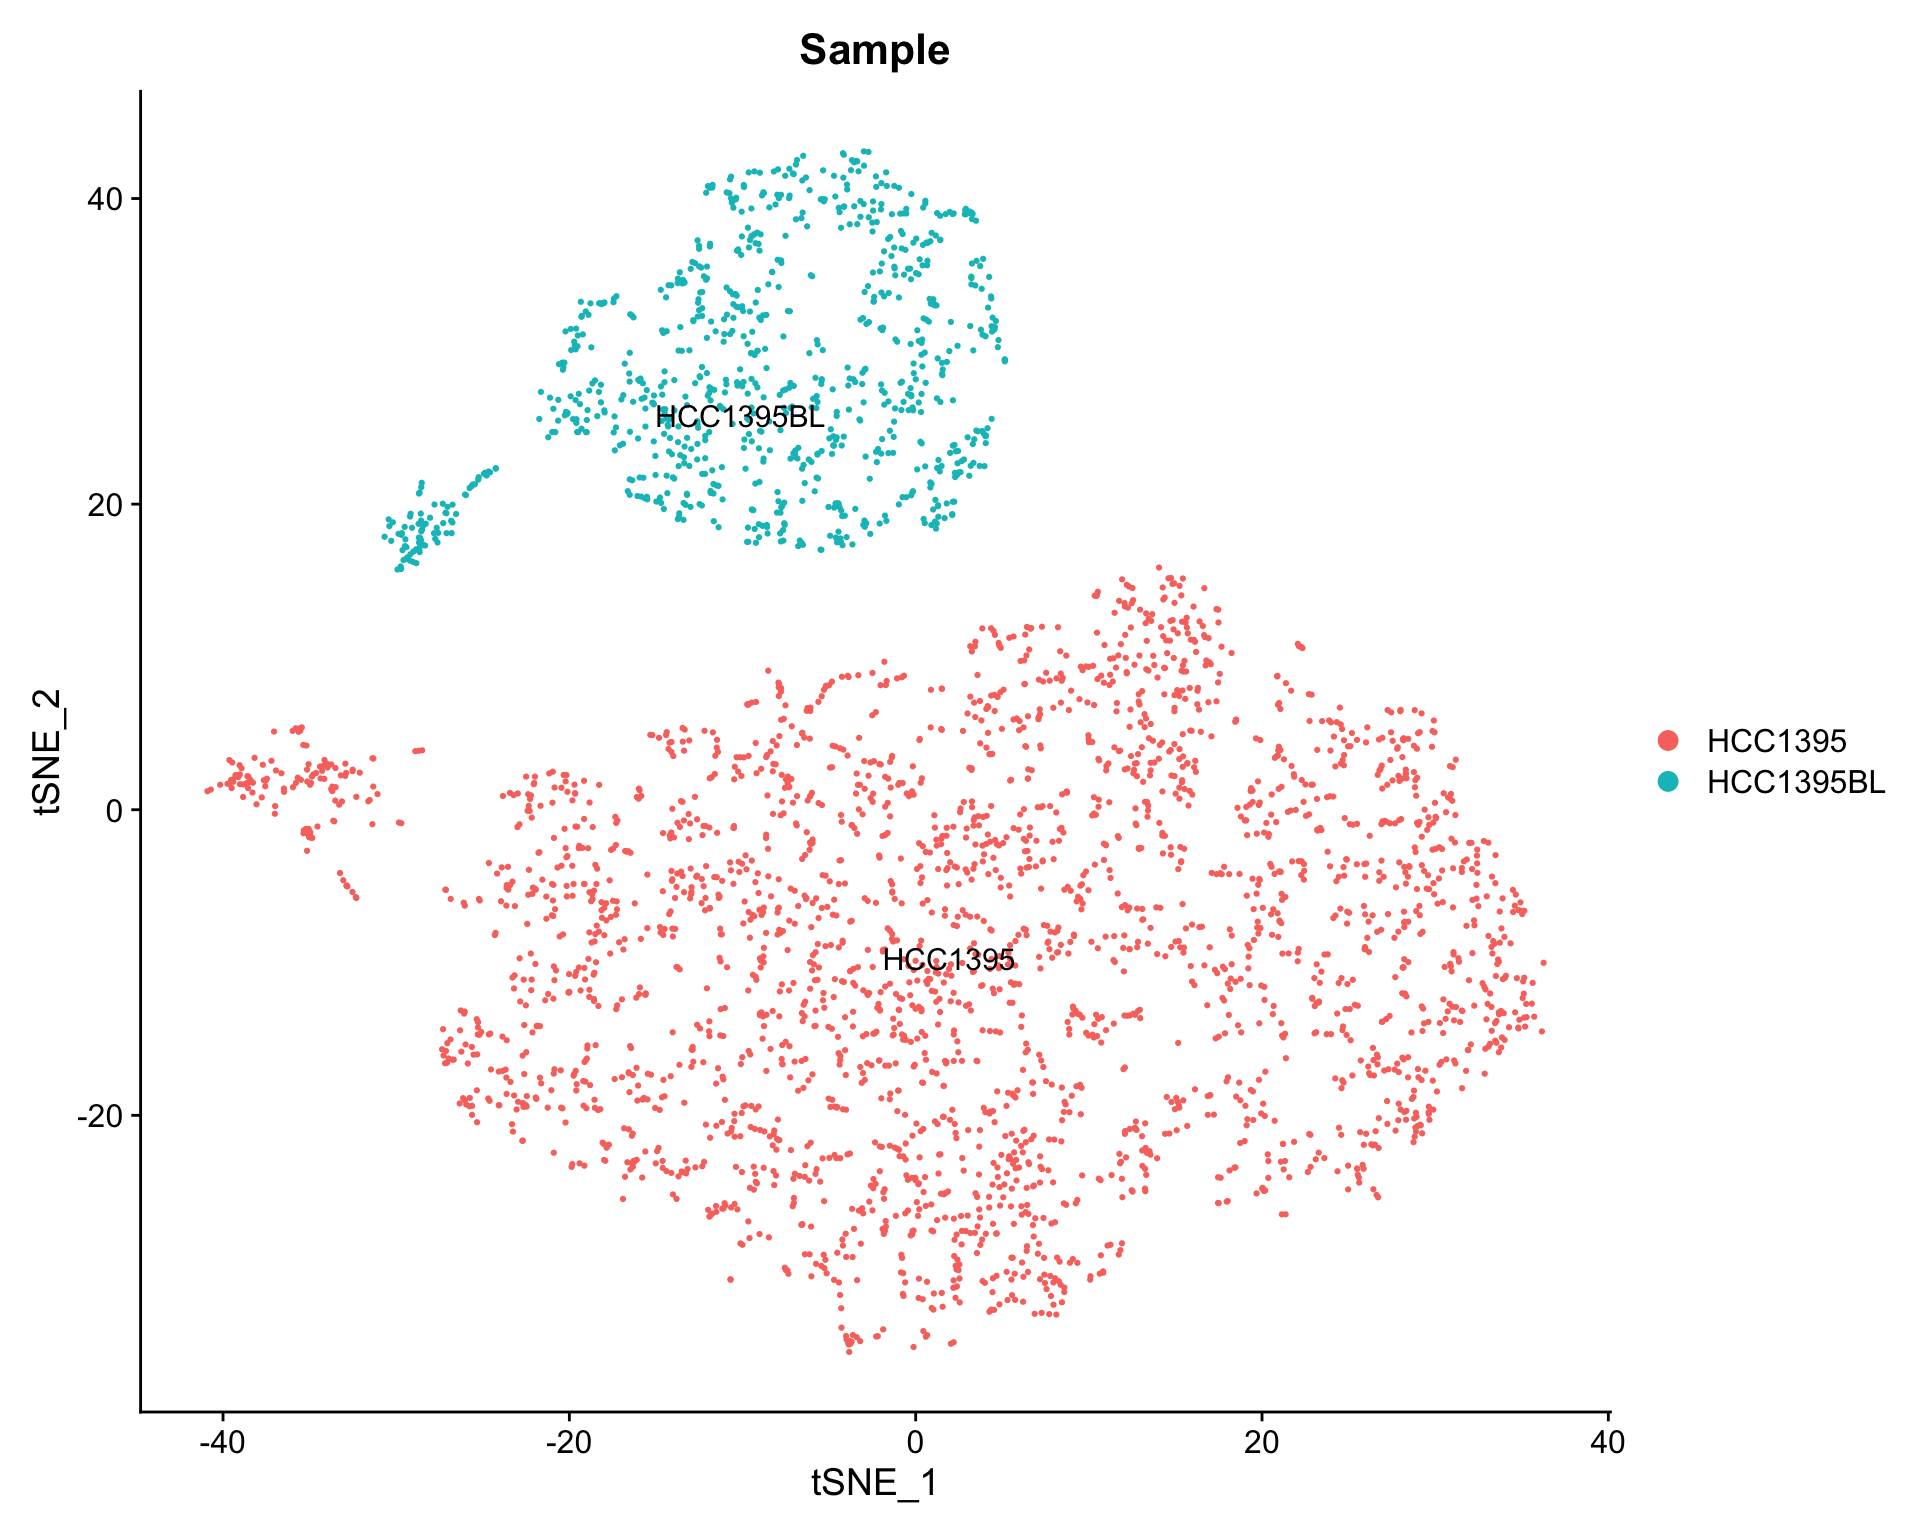
\includegraphics{scRNAseqtutorial_files/figure-latex/unnamed-chunk-43-1.pdf}

Optionally, we can also perform dimension reductionality reduction using UMAP

\begin{Shaded}
\begin{Highlighting}[]
\NormalTok{counts\_st }\OtherTok{\textless{}{-}} \FunctionTok{RunUMAP}\NormalTok{(counts\_st, }\AttributeTok{dims =} \DecValTok{1}\SpecialCharTok{:}\NormalTok{sel.dims,}\AttributeTok{verbose =}\NormalTok{ F)}
\end{Highlighting}
\end{Shaded}

\begin{verbatim}
## Warning: The default method for RunUMAP has changed from calling Python UMAP via reticulate to the R-native UWOT using the cosine metric
## To use Python UMAP via reticulate, set umap.method to 'umap-learn' and metric to 'correlation'
## This message will be shown once per session
\end{verbatim}

\begin{Shaded}
\begin{Highlighting}[]
\FunctionTok{DimPlot}\NormalTok{(}
\NormalTok{  counts\_st,}
  \AttributeTok{reduction =} \StringTok{"umap"}\NormalTok{,}
  \AttributeTok{label =}\NormalTok{ T,}
  \AttributeTok{size =} \FloatTok{0.5}\NormalTok{,}
  \AttributeTok{repel =}\NormalTok{ T,}
  \AttributeTok{cols =} \FunctionTok{DiscretePalette}\NormalTok{(}\FunctionTok{length}\NormalTok{(}\FunctionTok{levels}\NormalTok{(}\FunctionTok{Idents}\NormalTok{(}
\NormalTok{    counts\_st}
\NormalTok{  ))))}
\NormalTok{)}
\end{Highlighting}
\end{Shaded}

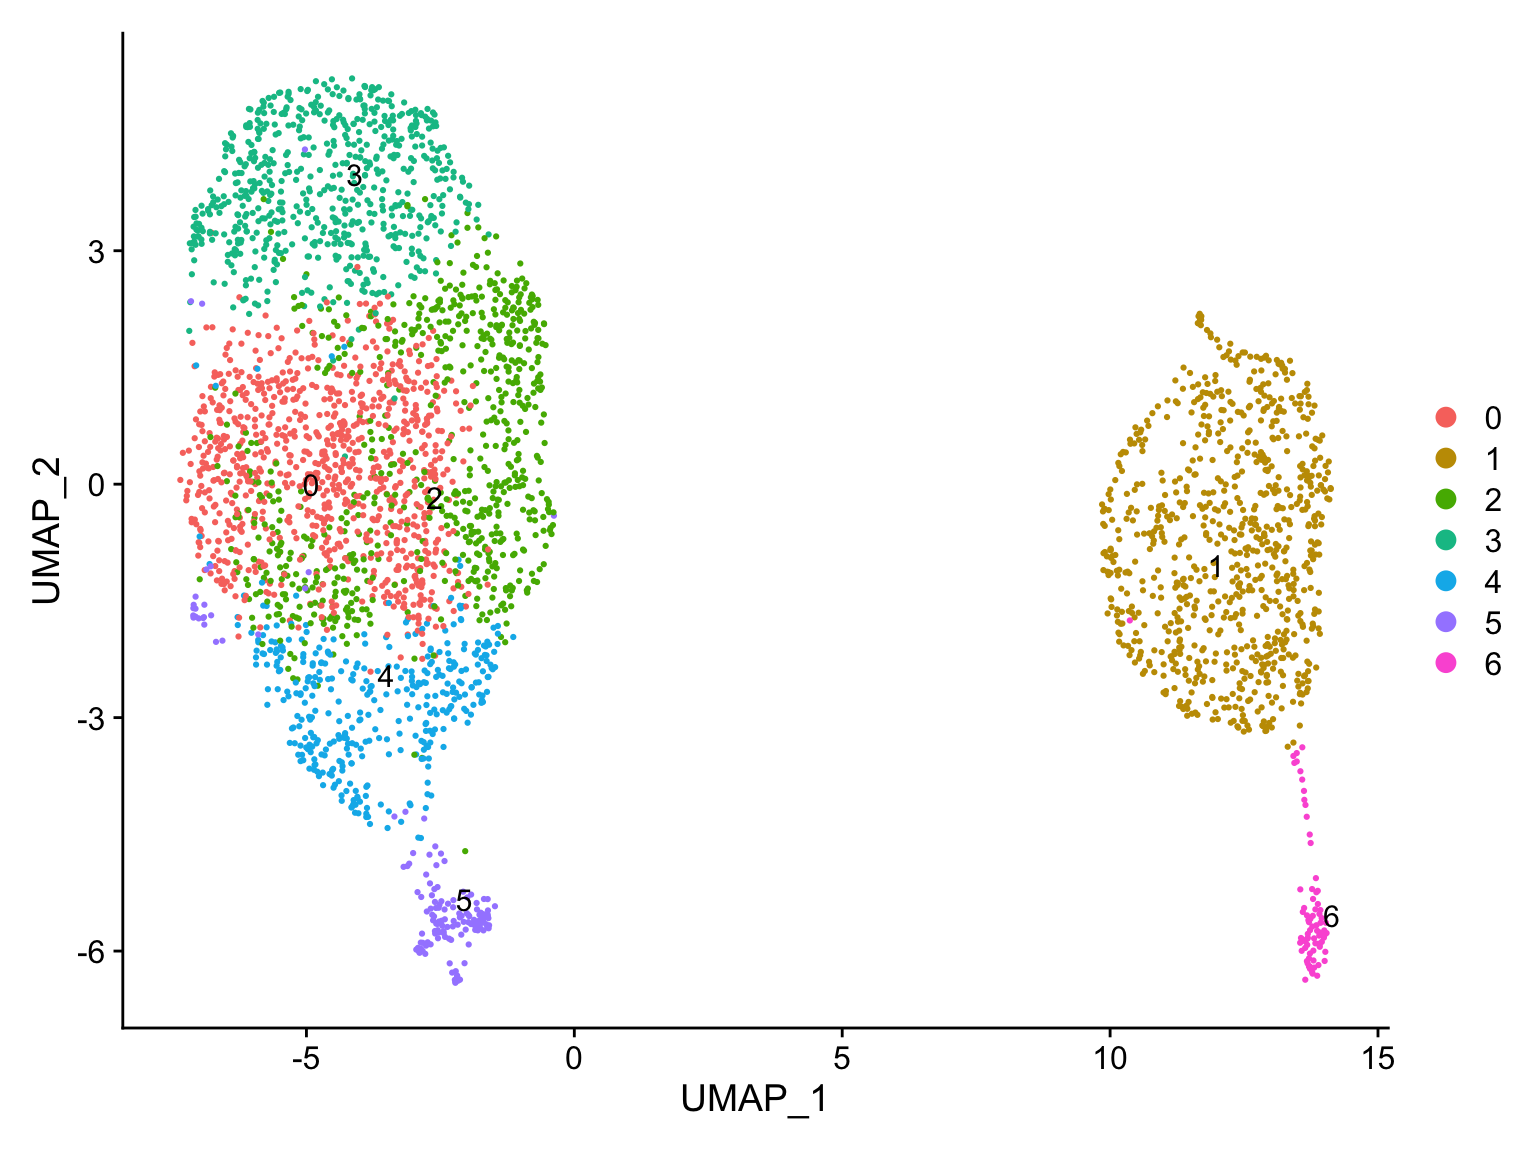
\includegraphics{scRNAseqtutorial_files/figure-latex/unnamed-chunk-44-1.pdf}

\begin{Shaded}
\begin{Highlighting}[]
\FunctionTok{DimPlot}\NormalTok{(}
\NormalTok{  counts\_st,}
  \AttributeTok{reduction =} \StringTok{"umap"}\NormalTok{,}
  \AttributeTok{label =}\NormalTok{ T,}
  \AttributeTok{group.by =} \StringTok{"Sample"}\NormalTok{,}
  \AttributeTok{size =} \FloatTok{0.5}\NormalTok{,}
  \AttributeTok{repel =}\NormalTok{ T}
\NormalTok{)}
\end{Highlighting}
\end{Shaded}

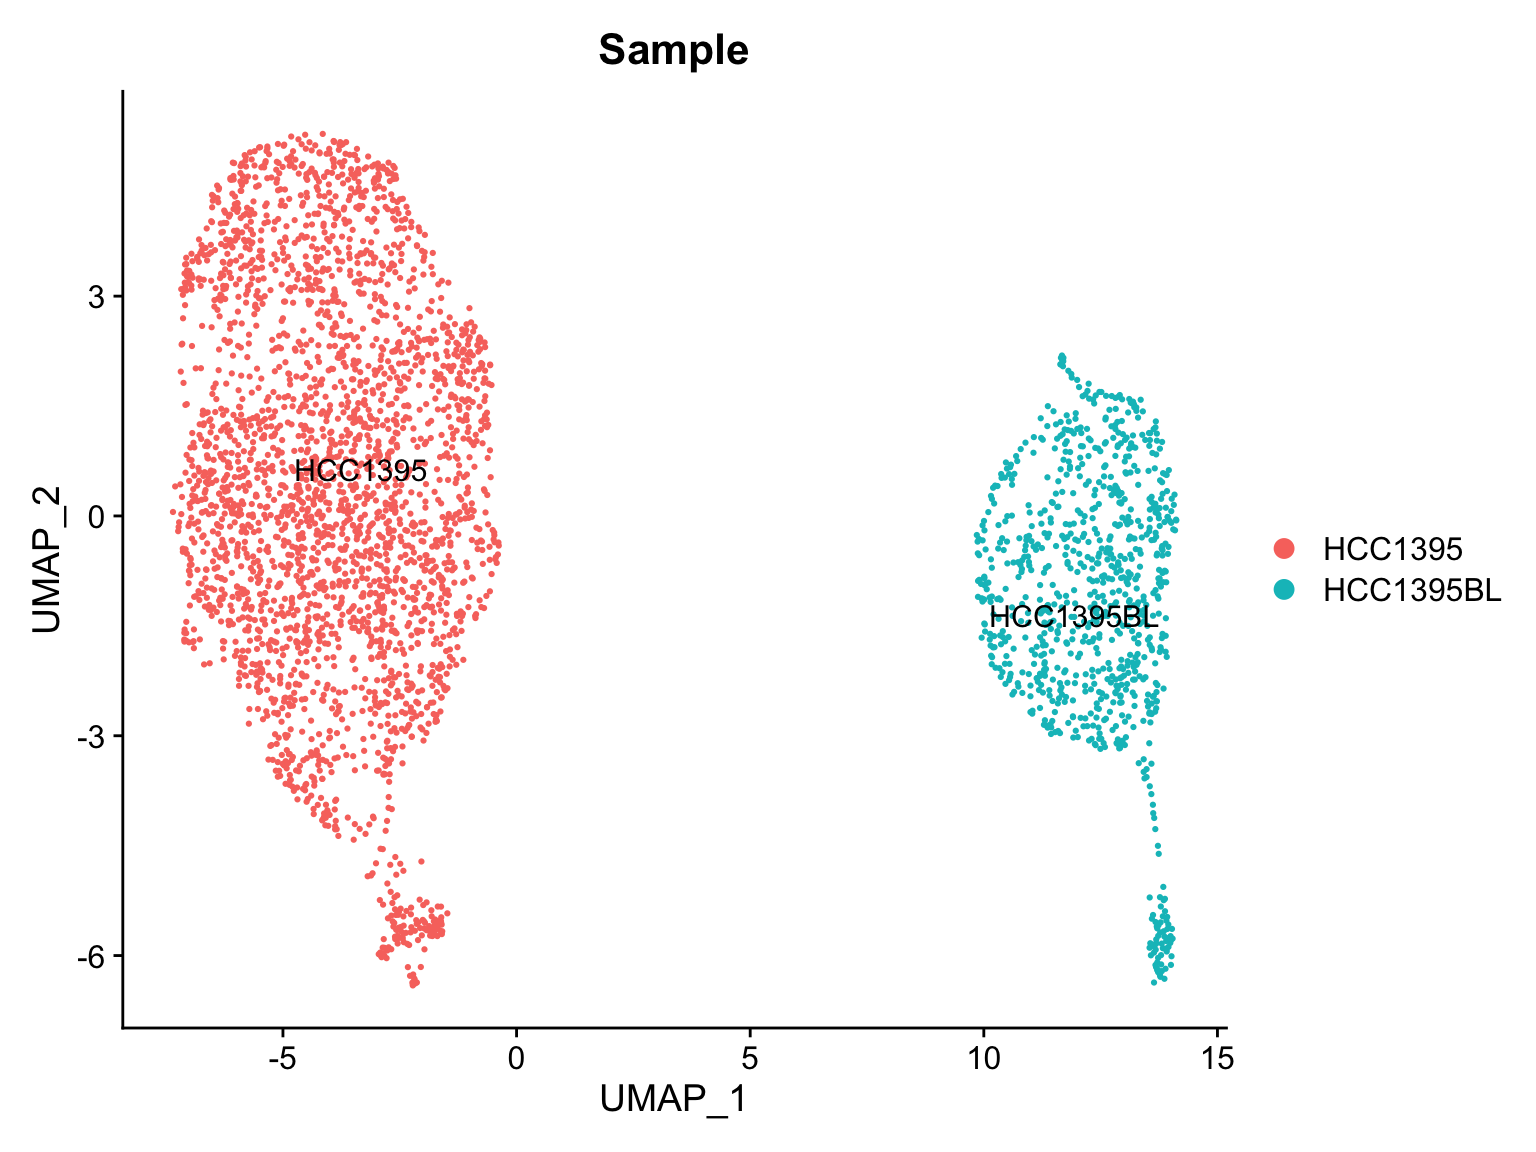
\includegraphics{scRNAseqtutorial_files/figure-latex/unnamed-chunk-45-1.pdf}
\#\# Differential expression analysis between clusters

To identify differentially expressed genes between clusters we can use the \emph{FindMarker} function in Seurat. As an example, DE genes between clusters 0 and 1 are computed below.

\begin{Shaded}
\begin{Highlighting}[]
\NormalTok{DE.cluster0\_1 }\OtherTok{\textless{}{-}} \FunctionTok{FindMarkers}\NormalTok{(counts\_st,}
                             \AttributeTok{ident.1 =} \DecValTok{0}\NormalTok{,}
                             \AttributeTok{ident.2 =} \DecValTok{1}\NormalTok{,}
                             \AttributeTok{verbose =}\NormalTok{ F)}
\FunctionTok{head}\NormalTok{(DE.cluster0\_1[}\FunctionTok{order}\NormalTok{(}\FunctionTok{abs}\NormalTok{(DE.cluster0\_1}\SpecialCharTok{$}\NormalTok{avg\_log2FC), }\AttributeTok{decreasing =}\NormalTok{ T), ])}
\end{Highlighting}
\end{Shaded}

\begin{verbatim}
##                p_val avg_log2FC pct.1 pct.2     p_val_adj
## CD74    0.000000e+00  -5.891577 0.008 1.000  0.000000e+00
## IGHM    0.000000e+00  -5.729445 0.000 0.998  0.000000e+00
## S100A6  0.000000e+00   5.598281 1.000 0.047  0.000000e+00
## TMSB4X 1.657565e-278  -4.911549 0.970 1.000 2.935713e-274
## CCL3   6.580286e-308  -4.861987 0.000 0.945 1.165434e-303
## KRT81  4.273972e-296   4.593045 0.962 0.000 7.569632e-292
\end{verbatim}

Marker genes which can be used to uniquely identify each of the clusters are identified using the \emph{FindAllMarkers} function.

\begin{Shaded}
\begin{Highlighting}[]
\NormalTok{all.markers}\OtherTok{\textless{}{-}}\FunctionTok{FindAllMarkers}\NormalTok{(counts\_st,}\AttributeTok{verbose =}\NormalTok{ F)}
\end{Highlighting}
\end{Shaded}

\begin{Shaded}
\begin{Highlighting}[]
\FunctionTok{library}\NormalTok{(dplyr)}
\NormalTok{all.markers }\SpecialCharTok{\%\textgreater{}\%}
    \FunctionTok{group\_by}\NormalTok{(cluster) }\SpecialCharTok{\%\textgreater{}\%}
    \FunctionTok{slice\_max}\NormalTok{(}\AttributeTok{n =} \DecValTok{5}\NormalTok{, }\AttributeTok{order\_by =}\NormalTok{ avg\_log2FC)}
\end{Highlighting}
\end{Shaded}

\begin{verbatim}
## # A tibble: 35 x 7
## # Groups:   cluster [7]
##        p_val avg_log2FC pct.1 pct.2 p_val_adj cluster gene   
##        <dbl>      <dbl> <dbl> <dbl>     <dbl> <fct>   <chr>  
##  1 1.61e-155      1.23  0.94  0.525 2.86e-151 0       IGFBP3 
##  2 4.07e- 65      1.17  0.417 0.149 7.21e- 61 0       IGFBP5 
##  3 2.12e-147      1.06  0.998 0.714 3.75e-143 0       TPM1   
##  4 2.31e-202      0.938 0.994 0.869 4.09e-198 0       CSNK2B 
##  5 1.78e-131      0.901 0.998 0.665 3.15e-127 0       TPM2   
##  6 0              4.79  0.998 0.021 0         1       IGHM   
##  7 0              4.63  1     0.037 0         1       CD74   
##  8 0              4.22  0.945 0.015 0         1       CCL3   
##  9 0              4.08  1     0.959 0         1       TMSB4X 
## 10 0              3.48  0.999 0.033 0         1       HLA-DRA
## # ... with 25 more rows
\end{verbatim}

\begin{Shaded}
\begin{Highlighting}[]
\NormalTok{top10.markers}\OtherTok{\textless{}{-}}\NormalTok{all.markers }\SpecialCharTok{\%\textgreater{}\%}
    \FunctionTok{group\_by}\NormalTok{(cluster) }\SpecialCharTok{\%\textgreater{}\%}
    \FunctionTok{slice\_max}\NormalTok{(}\AttributeTok{n =} \DecValTok{10}\NormalTok{, }\AttributeTok{order\_by =}\NormalTok{ avg\_log2FC)}
\end{Highlighting}
\end{Shaded}

\begin{Shaded}
\begin{Highlighting}[]
\FunctionTok{DoHeatmap}\NormalTok{(counts\_st, }\AttributeTok{features =}\NormalTok{ top10.markers}\SpecialCharTok{$}\NormalTok{gene)}
\end{Highlighting}
\end{Shaded}

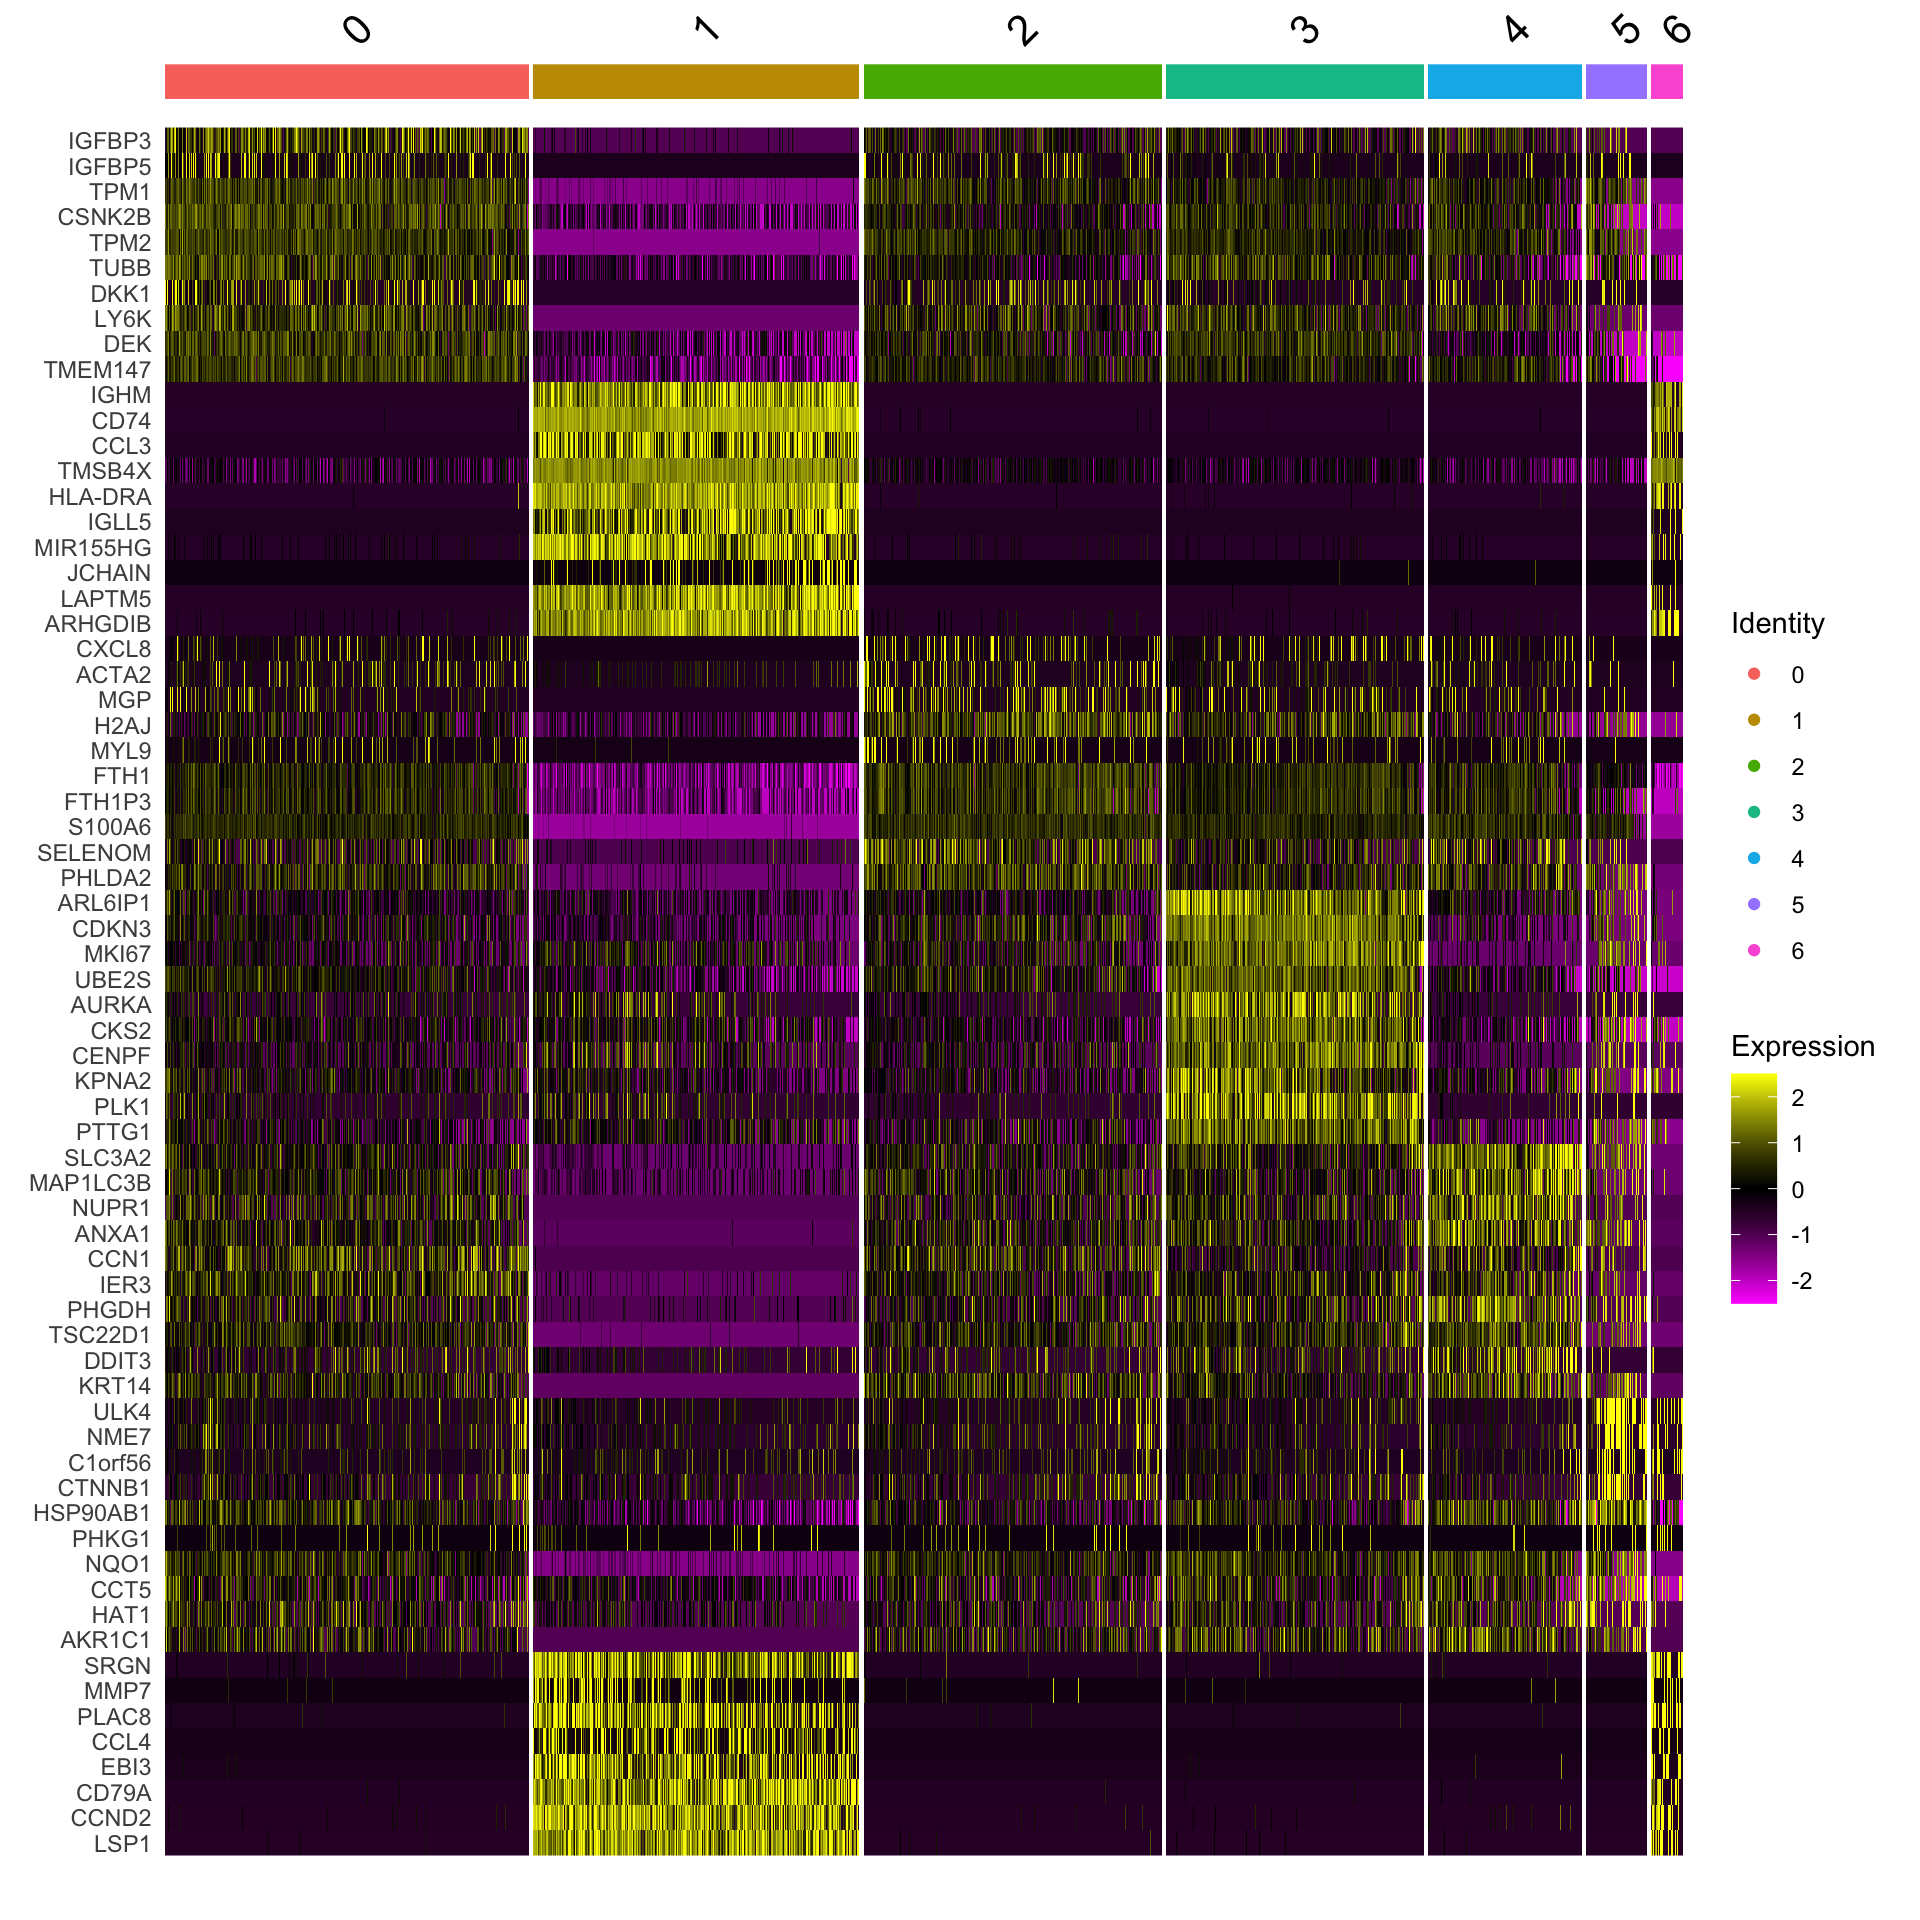
\includegraphics{scRNAseqtutorial_files/figure-latex/unnamed-chunk-51-1.pdf}

\hypertarget{cell-annotation}{%
\section{Cell annotation}\label{cell-annotation}}

An unbiased cell type recognition is performed using \textbf{SingleR}. \textbf{celldex} has a range of annotations derived from Bulk RNA-seq data that can be used to annotate the identified clusters above. Here, we use the Human Primary Cell Atlas database as an example.

\begin{Shaded}
\begin{Highlighting}[]
\FunctionTok{library}\NormalTok{(SingleR)}
\end{Highlighting}
\end{Shaded}

\begin{Shaded}
\begin{Highlighting}[]
\FunctionTok{library}\NormalTok{(SingleCellExperiment)}
\NormalTok{cell.sce}\OtherTok{\textless{}{-}} \FunctionTok{as.SingleCellExperiment}\NormalTok{(counts\_st)}
\NormalTok{annot}\OtherTok{\textless{}{-}}\NormalTok{celldex}\SpecialCharTok{::}\FunctionTok{HumanPrimaryCellAtlasData}\NormalTok{()}
\NormalTok{cell.annots }\OtherTok{\textless{}{-}} \FunctionTok{SingleR}\NormalTok{(}
    \AttributeTok{test =}\NormalTok{ cell.sce,}
    \AttributeTok{ref =}\NormalTok{ annot,}
    \AttributeTok{labels =}\NormalTok{ annot}\SpecialCharTok{$}\NormalTok{label.main)}

\NormalTok{cell.annots.fine}\OtherTok{\textless{}{-}}\FunctionTok{SingleR}\NormalTok{(}
    \AttributeTok{test =}\NormalTok{ cell.sce,}
    \AttributeTok{ref =}\NormalTok{ annot,}
    \AttributeTok{labels =}\NormalTok{ annot}\SpecialCharTok{$}\NormalTok{label.fine)}
\end{Highlighting}
\end{Shaded}

\begin{Shaded}
\begin{Highlighting}[]
\NormalTok{counts\_st }\OtherTok{\textless{}{-}}
  \FunctionTok{AddMetaData}\NormalTok{(counts\_st, cell.annots[}\FunctionTok{rownames}\NormalTok{(counts\_st}\SpecialCharTok{@}\NormalTok{meta.data), }\StringTok{"labels"}\NormalTok{], }\StringTok{"Annot.main"}\NormalTok{)}
\end{Highlighting}
\end{Shaded}

\begin{Shaded}
\begin{Highlighting}[]
\FunctionTok{DimPlot}\NormalTok{(}
\NormalTok{    counts\_st,}
    \AttributeTok{reduction =} \StringTok{"tsne"}\NormalTok{,}
    \AttributeTok{group.by =} \StringTok{"Annot.main"}\NormalTok{,}
    \AttributeTok{label =}\NormalTok{ T,}
    \AttributeTok{repel =}\NormalTok{ T,}
    \AttributeTok{pt.size =} \FloatTok{0.1}\NormalTok{,}
\NormalTok{  )}
\end{Highlighting}
\end{Shaded}

\begin{verbatim}
## Warning: ggrepel: 5 unlabeled data points (too many overlaps). Consider
## increasing max.overlaps
\end{verbatim}

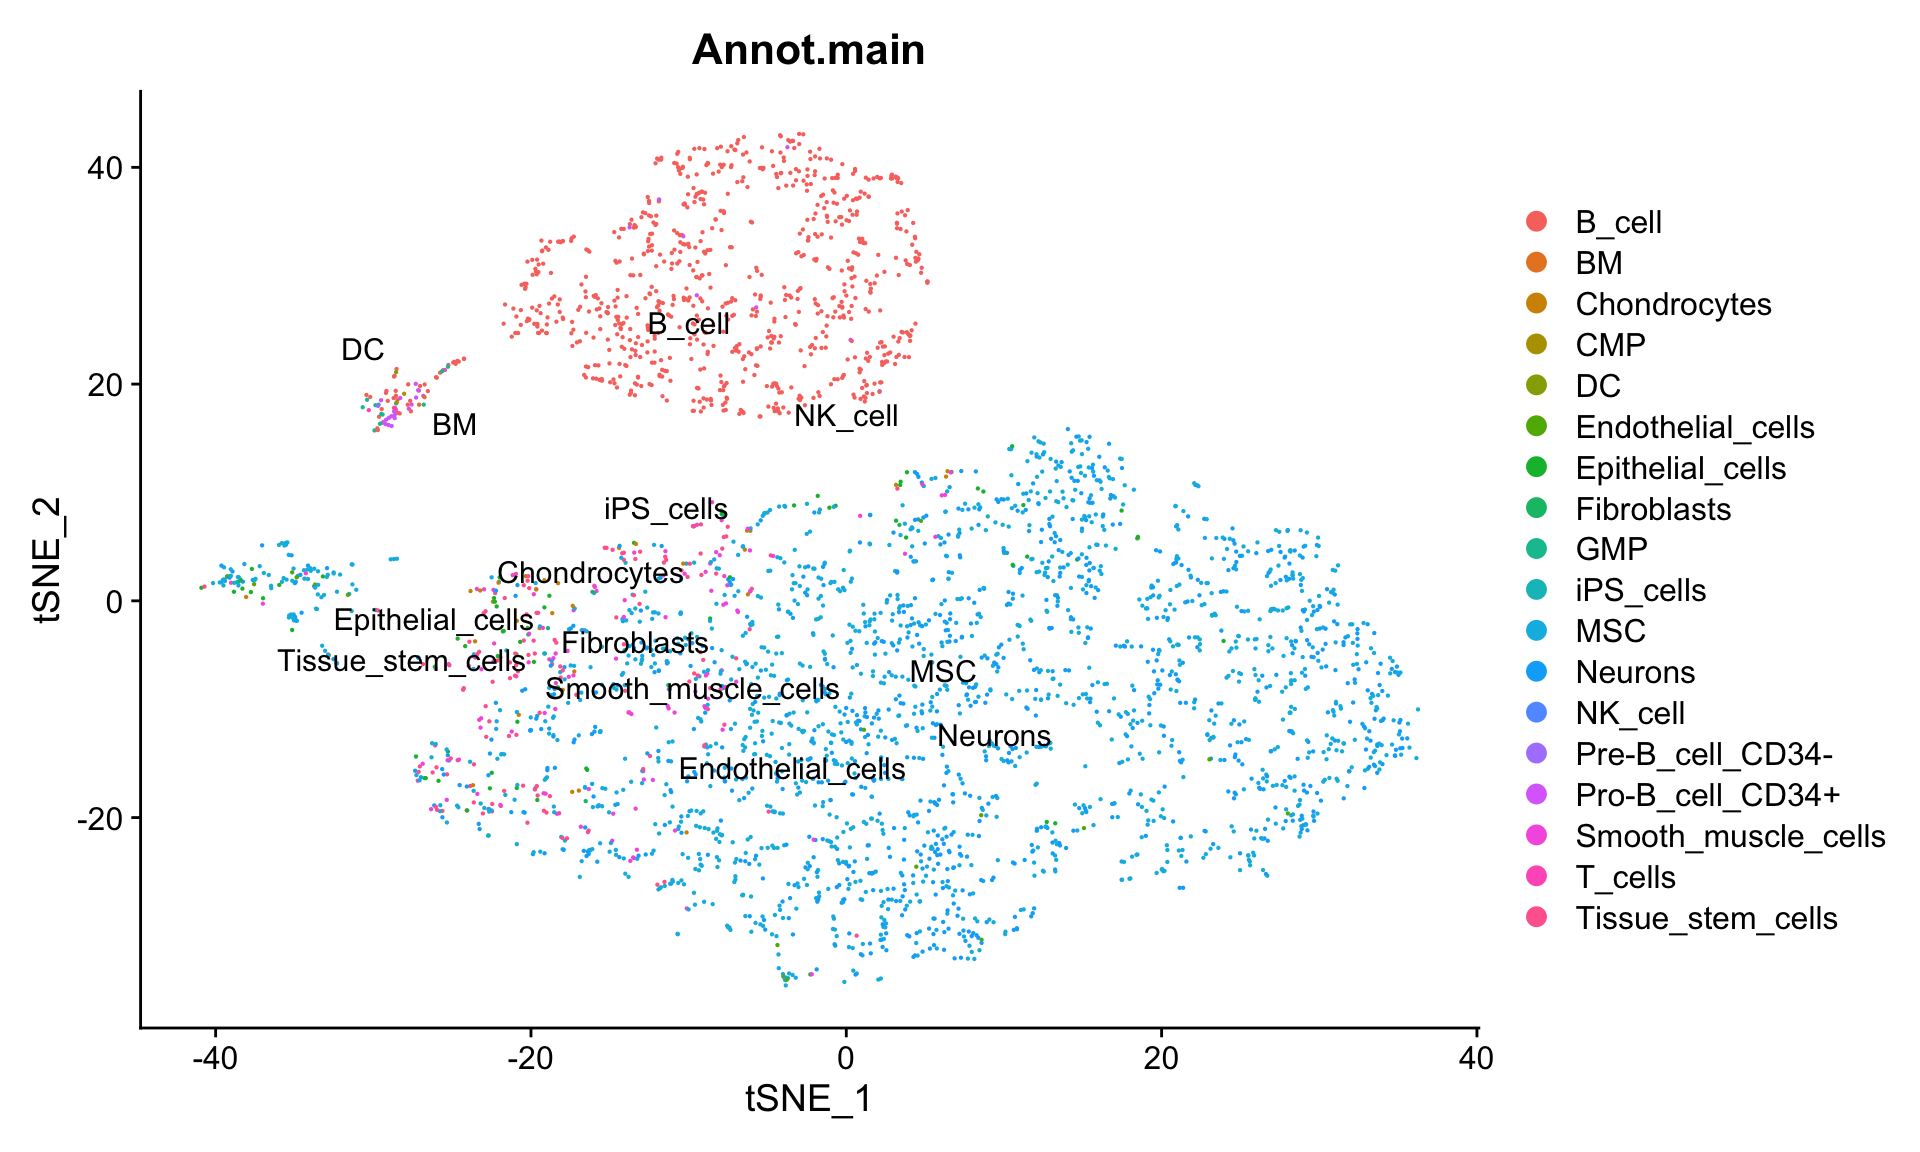
\includegraphics{scRNAseqtutorial_files/figure-latex/unnamed-chunk-56-1.pdf}

\begin{Shaded}
\begin{Highlighting}[]
\NormalTok{counts\_st }\OtherTok{\textless{}{-}}\FunctionTok{AddMetaData}\NormalTok{(counts\_st, cell.annots[}
  \FunctionTok{rownames}\NormalTok{(counts\_st}\SpecialCharTok{@}\NormalTok{meta.data), }\StringTok{"labels"}\NormalTok{], }\StringTok{"Annot.fine"}\NormalTok{)}
\end{Highlighting}
\end{Shaded}

\begin{Shaded}
\begin{Highlighting}[]
\FunctionTok{DimPlot}\NormalTok{(}
\NormalTok{    counts\_st,}
    \AttributeTok{reduction =} \StringTok{"tsne"}\NormalTok{,}
    \AttributeTok{group.by =} \StringTok{"Annot.fine"}\NormalTok{,}
    \AttributeTok{label =}\NormalTok{ T,}
    \AttributeTok{repel =}\NormalTok{ T,}
    \AttributeTok{pt.size =} \FloatTok{0.1}\NormalTok{)}
\end{Highlighting}
\end{Shaded}

\begin{verbatim}
## Warning: ggrepel: 5 unlabeled data points (too many overlaps). Consider
## increasing max.overlaps
\end{verbatim}

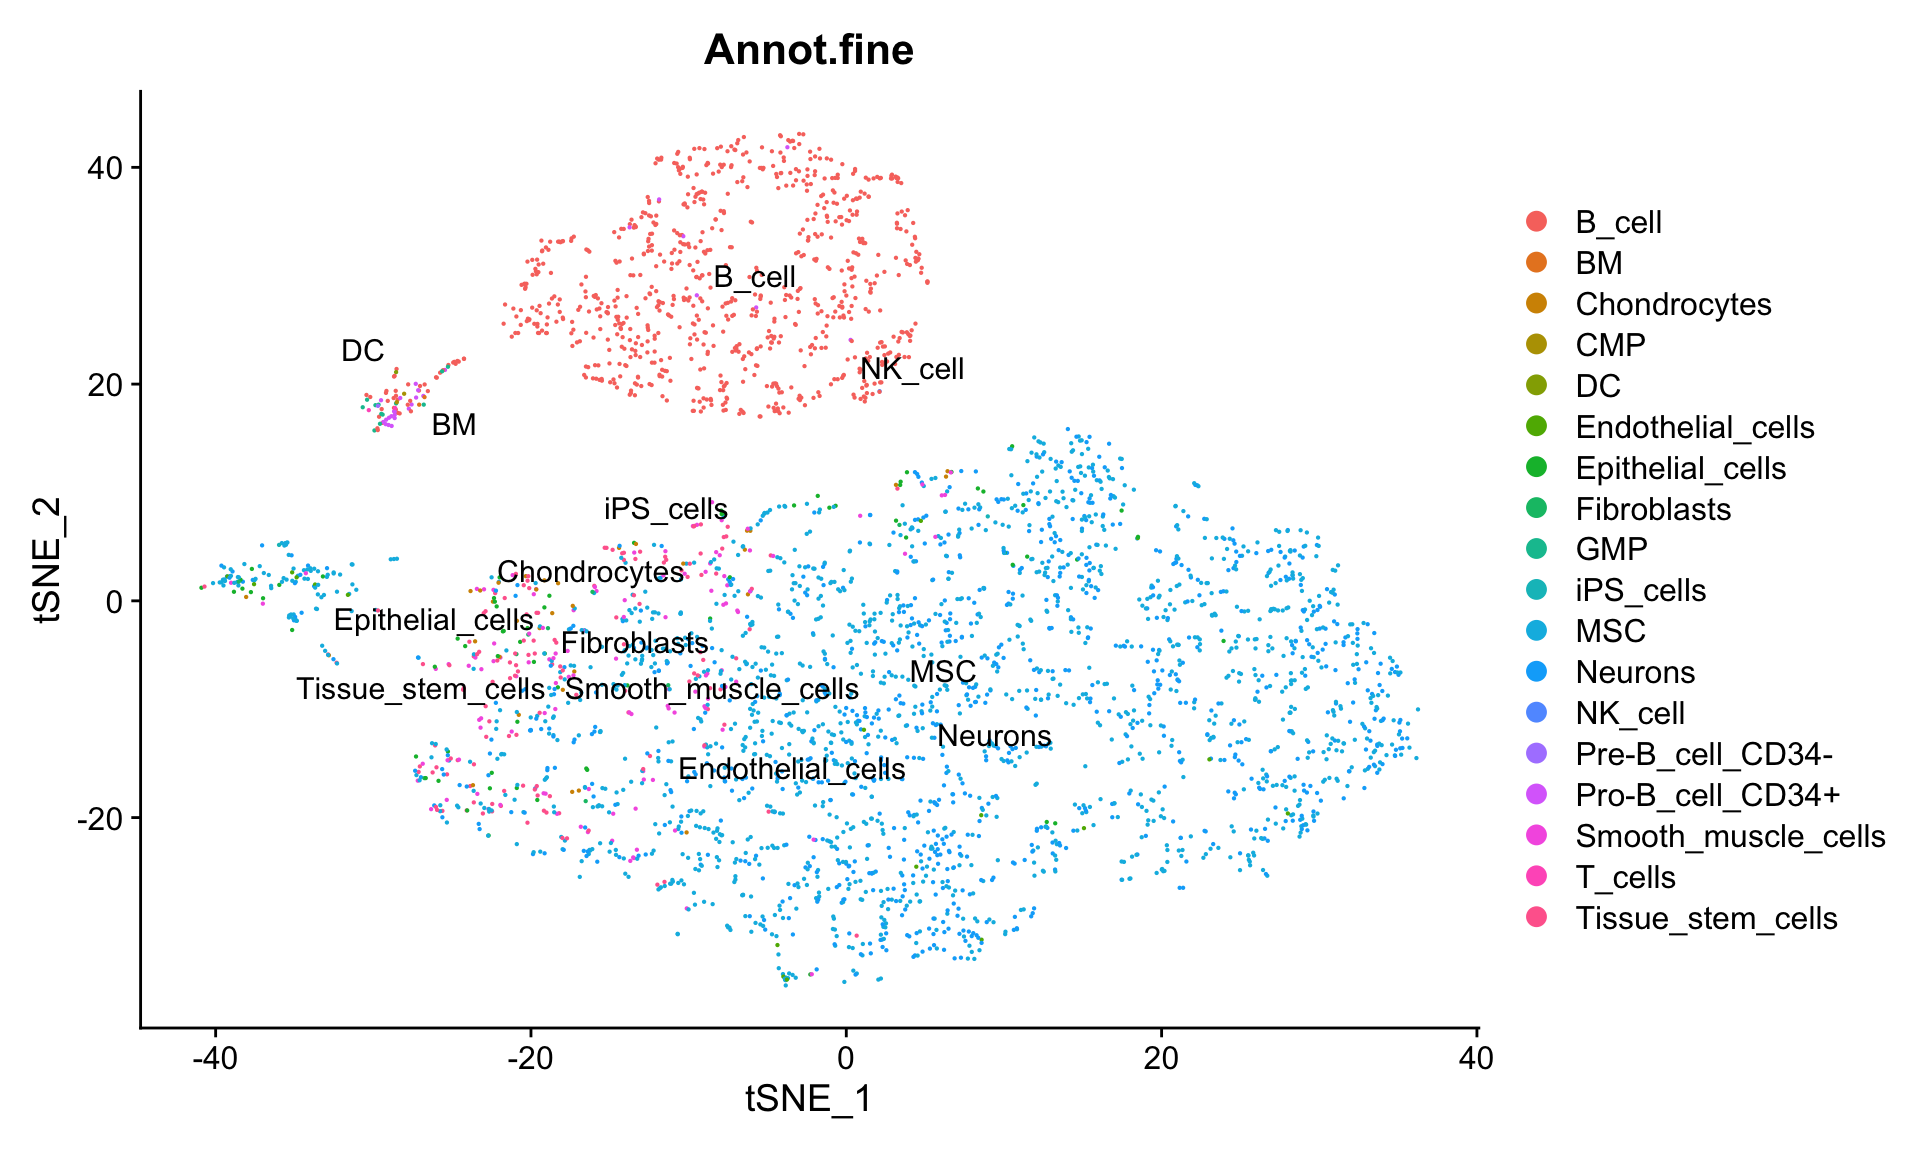
\includegraphics{scRNAseqtutorial_files/figure-latex/unnamed-chunk-58-1.pdf}

\hypertarget{trajectory-analysis}{%
\section{Trajectory analysis}\label{trajectory-analysis}}

Pseudotime analysis of the tuft cells identified in the dataset was performed using \textbf{Monocle2}.

\begin{Shaded}
\begin{Highlighting}[]
\NormalTok{mono2.learn.traject }\OtherTok{\textless{}{-}}
  \ControlFlowTok{function}\NormalTok{(X\_counts,}
\NormalTok{           these.cell.types) \{}
    \FunctionTok{library}\NormalTok{(monocle) }\CommentTok{\# It has to be Monocle 2.}
\NormalTok{    rds.fname }\OtherTok{\textless{}{-}}\StringTok{"Trajectory{-}cds.rds"}
\NormalTok{    gsndf }\OtherTok{\textless{}{-}} \FunctionTok{data.frame}\NormalTok{(}\AttributeTok{gene\_short\_name =} \FunctionTok{rownames}\NormalTok{(X\_counts))}
\NormalTok{    csndf }\OtherTok{\textless{}{-}} \FunctionTok{data.frame}\NormalTok{(}\AttributeTok{cell.type =}\NormalTok{ these.cell.types)}
    \FunctionTok{rownames}\NormalTok{(gsndf) }\OtherTok{\textless{}{-}} \FunctionTok{rownames}\NormalTok{(X\_counts)}
    \FunctionTok{rownames}\NormalTok{(csndf) }\OtherTok{\textless{}{-}} \FunctionTok{colnames}\NormalTok{(X\_counts)}
\NormalTok{    pd }\OtherTok{\textless{}{-}} \FunctionTok{new}\NormalTok{(}\StringTok{"AnnotatedDataFrame"}\NormalTok{, }\AttributeTok{data =}\NormalTok{ csndf)}
\NormalTok{    fd }\OtherTok{\textless{}{-}} \FunctionTok{new}\NormalTok{(}\StringTok{"AnnotatedDataFrame"}\NormalTok{, }\AttributeTok{data =}\NormalTok{ gsndf)}
\NormalTok{    cds }\OtherTok{\textless{}{-}}
      \FunctionTok{newCellDataSet}\NormalTok{(}
\NormalTok{        X\_counts,}
        \AttributeTok{phenoData =}\NormalTok{ pd,}
        \AttributeTok{featureData =}\NormalTok{ fd,}
        \AttributeTok{expressionFamily =} \FunctionTok{negbinomial.size}\NormalTok{()}
\NormalTok{      )}
\NormalTok{    cds }\OtherTok{\textless{}{-}} \FunctionTok{estimateSizeFactors}\NormalTok{(cds)}
\NormalTok{    cds }\OtherTok{\textless{}{-}} \FunctionTok{estimateDispersions}\NormalTok{(cds)}
\NormalTok{    cds }\OtherTok{\textless{}{-}} \FunctionTok{detectGenes}\NormalTok{(cds, }\AttributeTok{min\_expr =} \FloatTok{0.1}\NormalTok{)}
\NormalTok{    disp\_table }\OtherTok{\textless{}{-}} \FunctionTok{dispersionTable}\NormalTok{(cds)}
\NormalTok{    ordering\_genes }\OtherTok{\textless{}{-}} \FunctionTok{subset}\NormalTok{(disp\_table, mean\_expression }\SpecialCharTok{\textgreater{}=} \FloatTok{0.1}\NormalTok{)}
\NormalTok{    cds }\OtherTok{\textless{}{-}} \FunctionTok{setOrderingFilter}\NormalTok{(cds, ordering\_genes)}
\NormalTok{    cds }\OtherTok{\textless{}{-}} \FunctionTok{reduceDimension}\NormalTok{(cds)}
    \FunctionTok{saveRDS}\NormalTok{(cds , rds.fname)}
\NormalTok{\}}
\end{Highlighting}
\end{Shaded}

\begin{Shaded}
\begin{Highlighting}[]
\FunctionTok{mono2.learn.traject}\NormalTok{(}
  \AttributeTok{X\_counts =} \FunctionTok{as.matrix}\NormalTok{(counts\_st}\SpecialCharTok{@}\NormalTok{assays}\SpecialCharTok{$}\NormalTok{RNA}\SpecialCharTok{@}\NormalTok{counts),}
  \AttributeTok{these.cell.types =}\NormalTok{ counts\_st[[]]}\SpecialCharTok{$}\NormalTok{seurat\_clusters)}
\end{Highlighting}
\end{Shaded}

\begin{Shaded}
\begin{Highlighting}[]
\NormalTok{mono.rds }\OtherTok{\textless{}{-}}\FunctionTok{readRDS}\NormalTok{(}\StringTok{"Trajectory{-}cds.rds"}\NormalTok{)}
\NormalTok{mono.Tree }\OtherTok{\textless{}{-}} \FunctionTok{t}\NormalTok{(mono.rds}\SpecialCharTok{@}\NormalTok{reducedDimS)}
\end{Highlighting}
\end{Shaded}

\begin{Shaded}
\begin{Highlighting}[]
\NormalTok{do.Traj.lines }\OtherTok{\textless{}{-}} \ControlFlowTok{function}\NormalTok{(traj) \{}
  \ControlFlowTok{for}\NormalTok{ (i }\ControlFlowTok{in} \DecValTok{1}\SpecialCharTok{:}\FunctionTok{length}\NormalTok{(traj}\SpecialCharTok{@}\NormalTok{minSpanningTree[[]])) \{}
\NormalTok{    p1no }\OtherTok{\textless{}{-}} \FunctionTok{unlist}\NormalTok{(traj}\SpecialCharTok{@}\NormalTok{minSpanningTree[[i]])[}\DecValTok{1}\NormalTok{]}
\NormalTok{    p2no }\OtherTok{\textless{}{-}} \FunctionTok{unlist}\NormalTok{(traj}\SpecialCharTok{@}\NormalTok{minSpanningTree[[i]])[}\DecValTok{2}\NormalTok{]}
    \FunctionTok{lines}\NormalTok{(}
      \FunctionTok{c}\NormalTok{(traj}\SpecialCharTok{@}\NormalTok{reducedDimK[}\DecValTok{1}\NormalTok{, p1no],}
\NormalTok{        traj}\SpecialCharTok{@}\NormalTok{reducedDimK[}\DecValTok{1}\NormalTok{, p2no]),}
      \FunctionTok{c}\NormalTok{(traj}\SpecialCharTok{@}\NormalTok{reducedDimK[}\DecValTok{2}\NormalTok{, p1no],}
\NormalTok{        traj}\SpecialCharTok{@}\NormalTok{reducedDimK[}\DecValTok{2}\NormalTok{, p2no]),}
      \AttributeTok{lwd =} \DecValTok{2}
\NormalTok{    )}
\NormalTok{  \}}
\NormalTok{\}}
\end{Highlighting}
\end{Shaded}

\begin{Shaded}
\begin{Highlighting}[]
\NormalTok{clusters }\OtherTok{\textless{}{-}}\NormalTok{ counts\_st[[]]}\SpecialCharTok{$}\NormalTok{seurat\_clusters}
\NormalTok{cols.traj }\OtherTok{\textless{}{-}} \FunctionTok{c}\NormalTok{(}\StringTok{"red"}\NormalTok{, }\StringTok{"green"}\NormalTok{, }\StringTok{"blue"}\NormalTok{,}\StringTok{"orange"}\NormalTok{,}\StringTok{"purple"}\NormalTok{,}\StringTok{"pink"}\NormalTok{)}
\NormalTok{traj.cols }\OtherTok{\textless{}{-}}\NormalTok{  cols.traj[clusters]}
\FunctionTok{plot}\NormalTok{(}
\NormalTok{    mono.Tree,}
    \AttributeTok{cex =} \FloatTok{0.7}\NormalTok{,}
    \AttributeTok{pch =} \DecValTok{16}\NormalTok{,}
    \AttributeTok{bg =}\NormalTok{ traj.cols,}
    \AttributeTok{col =}\NormalTok{ traj.cols,}
    \AttributeTok{xlab =} \StringTok{"Component 1"}\NormalTok{,}
    \AttributeTok{ylab =} \StringTok{"Component 2"}\NormalTok{,}
    \AttributeTok{cex.axis =} \FloatTok{0.8}\NormalTok{,}
    \AttributeTok{cex.lab =} \FloatTok{0.9}
\NormalTok{)}
\FunctionTok{do.Traj.lines}\NormalTok{(mono.rds)}
\FunctionTok{legend}\NormalTok{(}
  \StringTok{"bottomright"}\NormalTok{,}
  \AttributeTok{legend =} \FunctionTok{levels}\NormalTok{(clusters),}
  \AttributeTok{pch =} \DecValTok{16}\NormalTok{,}
  \AttributeTok{col =}\NormalTok{ cols.traj,}
  \AttributeTok{bty =} \StringTok{"n"}
\NormalTok{)}
\end{Highlighting}
\end{Shaded}

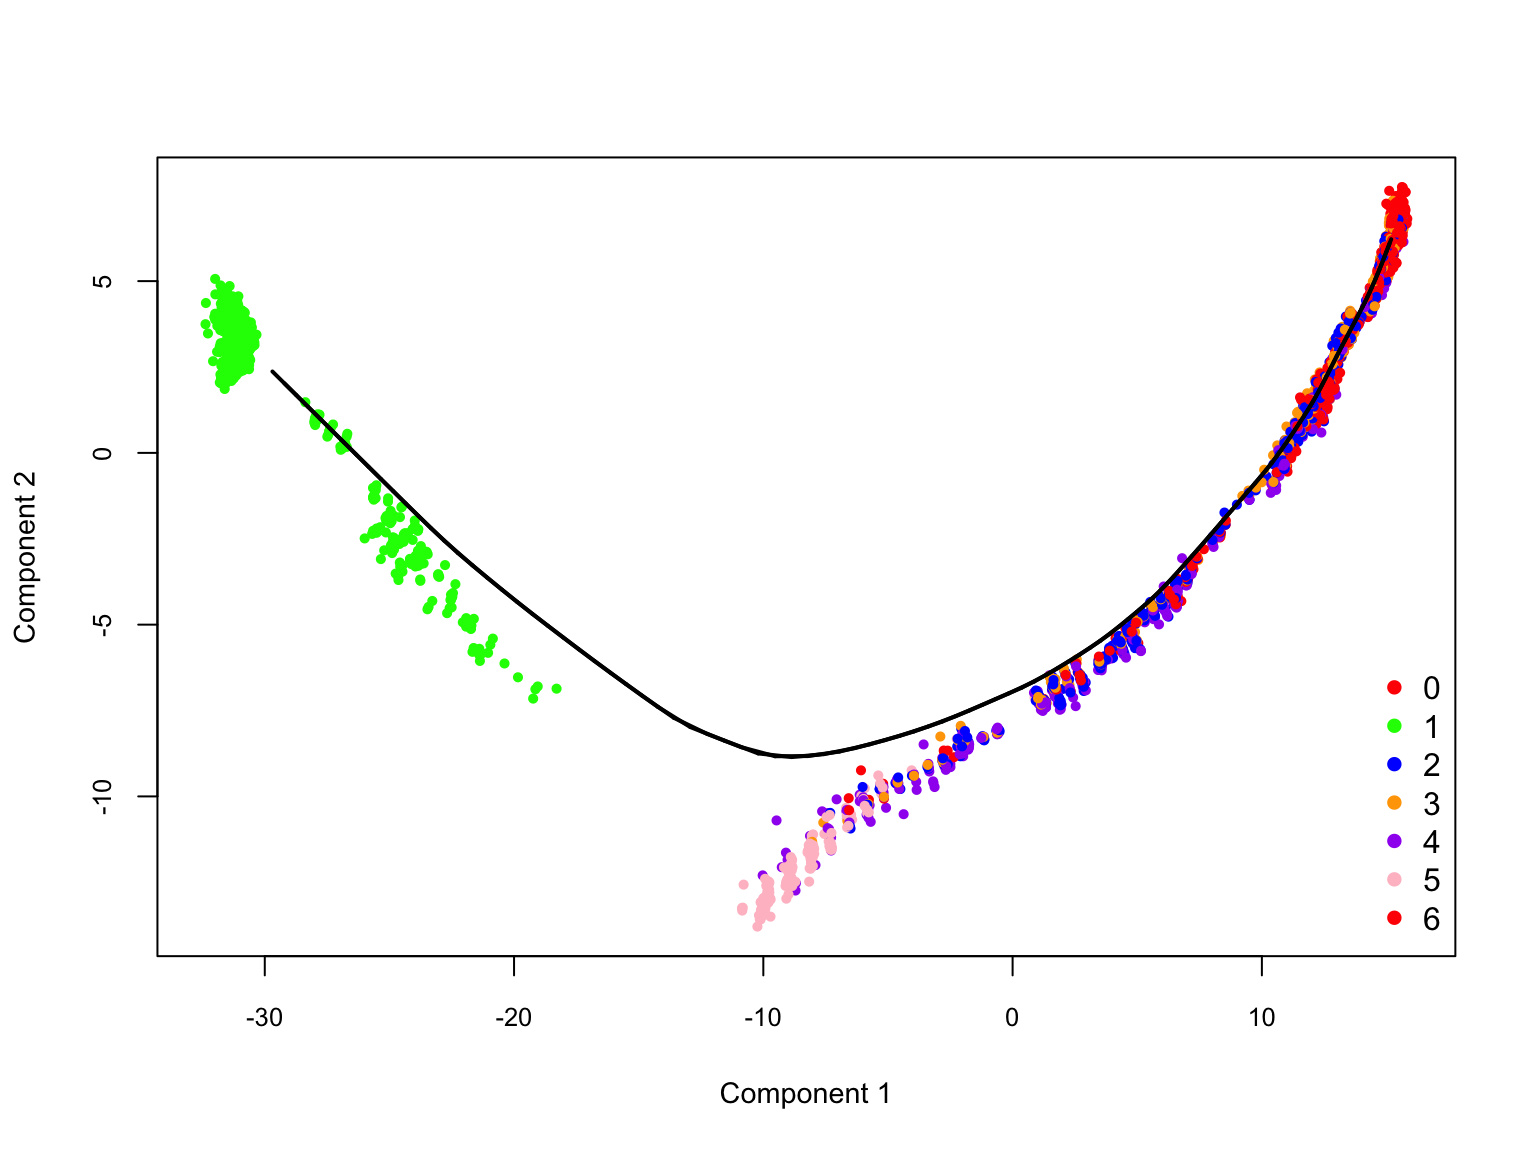
\includegraphics{scRNAseqtutorial_files/figure-latex/unnamed-chunk-63-1.pdf}

\textbf{Session info}

\begin{Shaded}
\begin{Highlighting}[]
\FunctionTok{sessionInfo}\NormalTok{()}
\end{Highlighting}
\end{Shaded}

\begin{verbatim}
## R version 4.2.0 (2022-04-22)
## Platform: x86_64-apple-darwin17.0 (64-bit)
## Running under: macOS Big Sur/Monterey 10.16
## 
## Matrix products: default
## BLAS:   /Library/Frameworks/R.framework/Versions/4.2/Resources/lib/libRblas.0.dylib
## LAPACK: /Library/Frameworks/R.framework/Versions/4.2/Resources/lib/libRlapack.dylib
## 
## locale:
## [1] en_AU.UTF-8/en_AU.UTF-8/en_AU.UTF-8/C/en_AU.UTF-8/en_AU.UTF-8
## 
## attached base packages:
## [1] stats4    stats     graphics  grDevices utils     datasets  methods  
## [8] base     
## 
## other attached packages:
##  [1] SingleR_1.10.0              SummarizedExperiment_1.26.1
##  [3] GenomicRanges_1.48.0        GenomeInfoDb_1.32.2        
##  [5] MatrixGenerics_1.8.0        matrixStats_0.62.0         
##  [7] dplyr_1.0.9                 org.Hs.eg.db_3.15.0        
##  [9] AnnotationDbi_1.58.0        IRanges_2.30.0             
## [11] S4Vectors_0.34.0            Biobase_2.56.0             
## [13] BiocGenerics_0.42.0         sp_1.5-0                   
## [15] SeuratObject_4.1.0          Seurat_4.1.1               
## [17] Rsubread_2.10.2            
## 
## loaded via a namespace (and not attached):
##   [1] plyr_1.8.7                igraph_1.3.2             
##   [3] lazyeval_0.2.2            splines_4.2.0            
##   [5] BiocParallel_1.30.3       listenv_0.8.0            
##   [7] scattermore_0.8           ggplot2_3.3.6            
##   [9] digest_0.6.29             htmltools_0.5.2          
##  [11] fansi_1.0.3               magrittr_2.0.3           
##  [13] memoise_2.0.1             ScaledMatrix_1.4.0       
##  [15] tensor_1.5                cluster_2.1.3            
##  [17] ROCR_1.0-11               limma_3.52.1             
##  [19] globals_0.15.0            Biostrings_2.64.0        
##  [21] spatstat.sparse_2.1-1     colorspace_2.0-3         
##  [23] blob_1.2.3                ggrepel_0.9.1            
##  [25] xfun_0.31                 crayon_1.5.1             
##  [27] RCurl_1.98-1.7            jsonlite_1.8.0           
##  [29] progressr_0.10.1          spatstat.data_2.2-0      
##  [31] survival_3.3-1            zoo_1.8-10               
##  [33] glue_1.6.2                polyclip_1.10-0          
##  [35] gtable_0.3.0              zlibbioc_1.42.0          
##  [37] XVector_0.36.0            leiden_0.4.2             
##  [39] DelayedArray_0.22.0       BiocSingular_1.12.0      
##  [41] future.apply_1.9.0        abind_1.4-5              
##  [43] scales_1.2.0              DBI_1.1.2                
##  [45] spatstat.random_2.2-0     miniUI_0.1.1.1           
##  [47] Rcpp_1.0.8.3              viridisLite_0.4.0        
##  [49] xtable_1.8-4              reticulate_1.25          
##  [51] spatstat.core_2.4-4       rsvd_1.0.5               
##  [53] bit_4.0.4                 htmlwidgets_1.5.4        
##  [55] httr_1.4.3                RColorBrewer_1.1-3       
##  [57] ellipsis_0.3.2            ica_1.0-2                
##  [59] farver_2.1.0              pkgconfig_2.0.3          
##  [61] uwot_0.1.11               deldir_1.0-6             
##  [63] utf8_1.2.2                labeling_0.4.2           
##  [65] tidyselect_1.1.2          rlang_1.0.2              
##  [67] reshape2_1.4.4            later_1.3.0              
##  [69] munsell_0.5.0             tools_4.2.0              
##  [71] cachem_1.0.6              cli_3.3.0                
##  [73] generics_0.1.2            RSQLite_2.2.14           
##  [75] ggridges_0.5.3            evaluate_0.15            
##  [77] stringr_1.4.0             fastmap_1.1.0            
##  [79] yaml_2.3.5                goftest_1.2-3            
##  [81] knitr_1.39                bit64_4.0.5              
##  [83] fitdistrplus_1.1-8        purrr_0.3.4              
##  [85] RANN_2.6.1                KEGGREST_1.36.2          
##  [87] sparseMatrixStats_1.8.0   pbapply_1.5-0            
##  [89] future_1.26.1             nlme_3.1-157             
##  [91] mime_0.12                 compiler_4.2.0           
##  [93] rstudioapi_0.13           plotly_4.10.0            
##  [95] png_0.1-7                 spatstat.utils_2.3-1     
##  [97] tibble_3.1.7              stringi_1.7.6            
##  [99] highr_0.9                 RSpectra_0.16-1          
## [101] rgeos_0.5-9               lattice_0.20-45          
## [103] Matrix_1.4-1              vctrs_0.4.1              
## [105] pillar_1.7.0              lifecycle_1.0.1          
## [107] spatstat.geom_2.4-0       lmtest_0.9-40            
## [109] BiocNeighbors_1.14.0      RcppAnnoy_0.0.19         
## [111] data.table_1.14.2         cowplot_1.1.1            
## [113] bitops_1.0-7              irlba_2.3.5              
## [115] httpuv_1.6.5              patchwork_1.1.1          
## [117] R6_2.5.1                  bookdown_0.27            
## [119] promises_1.2.0.1          KernSmooth_2.23-20       
## [121] gridExtra_2.3             parallelly_1.32.0        
## [123] codetools_0.2-18          MASS_7.3-57              
## [125] assertthat_0.2.1          withr_2.5.0              
## [127] sctransform_0.3.3         GenomeInfoDbData_1.2.8   
## [129] mgcv_1.8-40               parallel_4.2.0           
## [131] beachmat_2.12.0           grid_4.2.0               
## [133] rpart_4.1.16              tidyr_1.2.0              
## [135] DelayedMatrixStats_1.18.0 rmarkdown_2.14           
## [137] Rtsne_0.16                shiny_1.7.1
\end{verbatim}

\vspace{-100pt}

  \bibliography{Genome.bib,packages.bib}

\end{document}
